\documentclass[british,titlepagevegard,oneside]{ntnuthesis}

\newcommand{\todo}[1]{\textcolor{red}{TODO: {#1}}}

\title{Comparison of two classical landmark detectors for side scan sonars}
\shorttitle{Comparison of landmark detectors}
\author{Vegard Haraldstad}
\shortauthor{Haraldstad}
\date{\today}

\addtolength{\oddsidemargin}{-.875in}
\addtolength{\evensidemargin}{-.875in}
\addtolength{\textwidth}{1.75in}

\addbibresource{thesis.bib}

%\input{glossary.tex} % add glossary and acronym lists before document

\begin{document}

\chapter*{Abstract}

This report tests two landmark detection methods using side scan sonar (SSS) and presents a novel quality indicator for assessing SSS data in terms of its information content. The report moreover provides an overview of the advantages and drawbacks of the two methods and strives for finding which one of the methods is the most promising for the purpose of implementing a feature-based Simultaneous Localization and Mapping (SLAM) pipeline. In the process, the report comments on the fact that robust landmark detection (i.e., detection that is invariant to changing environments) is an enabling factor for obtaining accurate feature-based SLAM. 

For this, we note that current methods primarily rely on deep learning or classical strategies such as shadow and/or echo detection. However, to the best of our knowledge, the available research does not extensively test different methods against each other; it is therefore difficult to judge what is best when. To address this, this report tests two classical methods on SSS data collected from the Trondheim fjord and qualitatively compares them against each other. In more detail, the first method uses peak detection to find shadows and echoes in 1D sonar swaths. The second method instead finds shadows in 2D sonar images using expert rules. The results show that both methods lack robustness and, to a varying degree, cannot consistently detect landmarks.

For the purpose of carrying on the analysis above in the most rigorous way possible, we propose a dedicated quality indicator that uses the raw information available from the sensors to assess the quality of the data they have been producing. This quality indicator is based on assessing the amount of overlapping of consecutive swaths and does so for the ground range at the maximum sensor opening. Therefore, the proposed index only reports on overlapping in the ranges we expect to find valuable information. However, it does not directly consider changes in speed and angles and thus is not able to detect (and thus indicate) poor quality when anomalies in the data occur from changing speed or roll angle. 


\tableofcontents
%\listoffigures
%\listoftables
%\lstlistoflistings

%\printglossary[type=\acronymtype] % Print acronyms
%\printglossary                    % Print glossary

\chapter{Introduction}

As the population grows, utilizing the resources and areas in and on the ocean becomes more critical, as resources and land space are limited and in great demand. It is expected a large increase in both green energy and aquaculture production in the future \cite{Oceans2050}. Recent examples are the offshore wind farms Hywind Tampen \cite{HywindEquinor} and the offshore fish farming project Ocean Farm 1\cite{HavbasertASA}. Deep sea mining is also an up-and-coming market, with the potential to provide rear-earth metals for producing, for example, electronic devices and vehicles \cite{Bogue2015UnderwaterApplications}.

To make use of the ocean, one crucial aspect is monitoring the fragile ecosystems and the installed infrastructure. Monitoring the ecosystems is essential, ensuring that our activity in the sea is sustainable and does not destroy fragile ecosystems. Fish farming in the fjords has proven to put the ecosystems out of balance; for example, how salmon lice threaten the wild salmon swimming in the same area as the fish farms and how the waste from fish farming affects the ecosystem in the ocean \cite{Fiskeoppdrett}. Further, there have been worries about the impact on the ecosystems deep sea mining can have \cite{UnderstandingTechnology}. On the other side, monitoring and maintaining the installed infrastructure is crucial from an economic perspective. A typical operation is to inspect subsea pipelines and cables, ensuring they have not moved and are in good shape. 

AUVs are used for monitoring and surveying the ocean \cite{Nicholson2008TheTechnologies}, \cite{HaugstadDenManeder}. They are often more cost-effective than manned vessels and, in addition, more environmentally friendly. Even though they are used in commercial applications, they still have some challenges constraining their operational areas. Such challenges include underwater navigation and communication, making long-time operations without surfacing challenging. 

One of the most significant challenges for doing long-time AUV operations is that electromagnetic waves have constraints in their use underwater, making GNSS unavailable and, in practice restricting communication to acoustic communication with low bandwidth for submerged AUVs \cite{Nicholson2008TheTechnologies}. This makes long-term autonomous operations difficult. The restriction of communication restricts the possibilities for monitoring and human supervision, making the AUV more dependent on its autonomous capabilities. One key element for this is reliable and accurate navigation and localization. Without GNSS, reliable localization either needs expensive inertial sensors or an external position system, such as acoustic beacons for localization, that is expensive to install and restricts the operating area. A promising solution is simultaneous localization and mapping (SLAM).

SLAM has significantly impacted mobile robotics, improving the localization and mapping of unknown environments. It has, for example, been applied to drones \cite{VonStumberg2017FromExploration}, where a camera is typically used to provide the perception of the environment. In underwater applications, SLAM has also been utilized \cite{Hidalgo2015ReviewTechniques}. However, using a camera underwater is problematic because of the turbidity in the water and the lack of light at greater depths, significantly reducing sight, so the method used above water can not be directly ported to the underwater domain \cite{Paull2015Communication-constrainedSLAM}.  

Another way to observe the underwater environment is to use sonar, a sensor that uses acoustics to sense its surroundings. A sonar transmits acoustic pulses and "senses" the echoes reflected from its environment to give a perception of the environment. A great advantage over cameras is that it is not affected by turbidity and light conditions, making sonar an excellent alternative for underwater applications. Because of this, much of the research available focuses on SLAM using sonars to perform long-time operations without additional measures \cite{Hidalgo2015ReviewTechniques}.

\section{Project Description}

This project aims to test two landmark detection methods using side scan sonar (SSS). It provides an overview of the advantages and drawbacks of the different techniques for finding the most promising method to use in a feature-based Simultaneously Localization and Mapping (SLAM) pipeline. Further, it presents a novel quality indicator for SSS data.

The work has been done under the supervision of Simon Andreas Hagen Hoff and Damiano Varagnolo, and their insight and help have been greatly appreciated. Thanks to Tore Mo-Bjørkelund and Ambjørn Waldum for providing side scan sonar data and insight into how the data was acquired. 

\section{Report structure}

First, this report will present the background needed for context and understanding of the work in this report. Secondly, the landmark detectors and the quality indicator will be presented together with an explanation of how the results are considered. Thirdly, the results of running the landmark detectors and the quality indicator on side scan sonar data are presented. Last, a discussion about the landmark detectors and the quality indicator, their performance, weaknesses, and strengths, together with a comparison of the two landmark detectors.  



\chapter{Background}

This chapter will present the relevant background for this report. 

\section{Simultaneous localization and mapping}

Simultaneous localization and mapping (SLAM) is a procedure of acquiring a map of an unknown environment as a mobile platform explores it and, at the same time, localizes the mobile platform on the same map, and it is one of the key enabling technologies of mobile robot navigation \cite{Stachniss2016SimultaneousMapping}. More technically, SLAM is the procedure of estimating the sequence of robot poses, or the robot path, $X_t = \{x_0, x_1, x_2,...,x_t\}$, where $t$ denotes the time. The robot uses different sensors and/or motion models to obtain its odometry, $U_t = \{u_0, u_1, u_2,...,u_t\}$, describing the relative motion between time $t-1$ and $t$. Further, the robot uses sensors to sense the environment. The environment can be either modeled by volumetric or feature-based models. The volumetric model has a high enough resolution that allows for photo-realistic reconstruction and is a high-dimensional problem. Feature-based or landmark-based models are of a lower dimension and tend to be faster. Since this report tests landmark detectors, only feature-based SLAM is treated further. Let the pose of landmark $n$ be denoted $l_n$. Then, the robot measures the relative position between its pose, $x_t$, and the landmark poses of the landmarks in map $m$. Let the vector containing all landmark measurements at time $t$ be denoted $z_t$. The measurement of landmarks is then given by $Z_t = \{z_0, z_1, z_2,...,z_t\}$.

Factor graphs are the de-facto standard for modeling SLAM. The nodes in the graph represent the robot poses and the landmark positions, and the factors represent the odometry and landmark measurements. \cref{fig:factor_graph} shows a simple SLAM problem with four poses, $x_t$, and two landmarks, $l_n$. The odometry, $u_t$, between two consecutive poses is given by

\begin{equation}
    u_t = p(x_t \,|\, x_{t-1},u_t),
    \label{eq:odom_pdf}
\end{equation}

and landmark measurements, $z_{t,n}$ of landmark $n$ at time $t$ is given as

\begin{equation}
    z_{t,n} = p(z_{t,n} \,|\, x_{t-1},m).
    \label{eq:landmark_measurement_pdf}
\end{equation}

Using the factor graph formulation, the SLAM problem can be formulated as a maximum a posteriori (MAP) estimation, where the goal is to estimate the path, $X_t$, and map, $m$, that maximizes the likelihood given by

\begin{equation}
    X_t^*, m^* = \argmax_{X_t,m} \, logp(X_t,m \,|\, Z_t,U_t),
    \label{eq:SLAM}
\end{equation}

which is also often called the back-end of SLAM.

The front-end of SLAM consists of landmark detection and data association. Landmark detection is the procedure of finding and detecting landmarks from the sensors sensing the environment, for example, a camera.  Data association is the procedure of determining the landmark identity of the detected landmarks.

\begin{figure} [t]
    \centering
    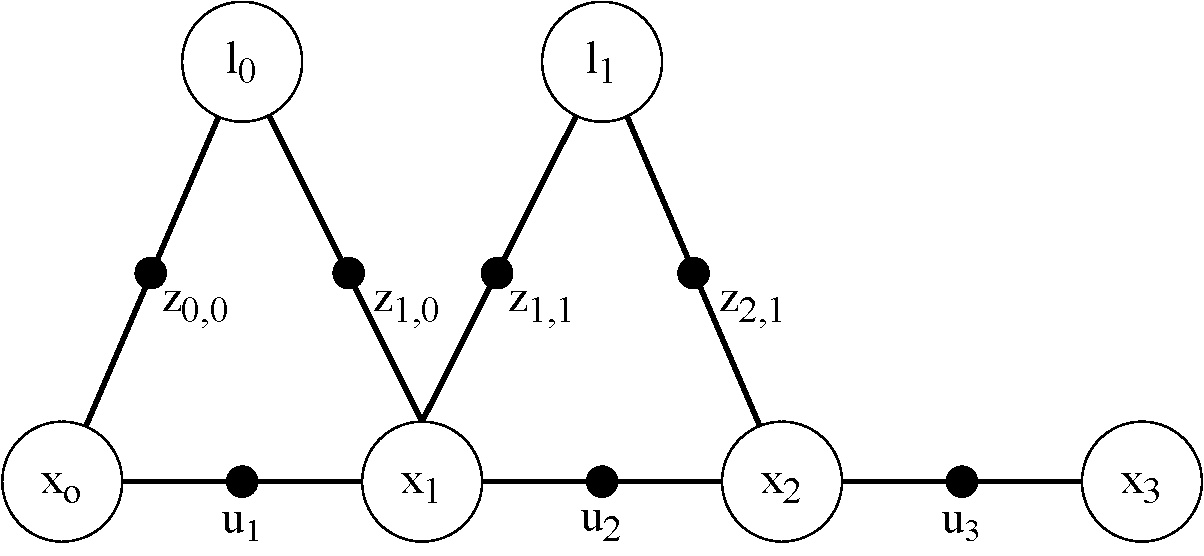
\includegraphics[width=0.6\textwidth]{figures/factor_graph.drawio.pdf}
    \caption{Factor graph of a simple SLAM problem containing four poses and two landmarks.}
    \label{fig:factor_graph}
\end{figure}


Underwater SLAM is a challenging research topic, and task for underwater vehicles in long-term operation due to the limitations of subsea localization sensors and perception sensors for mapping \cite{Hidalgo2015ReviewTechniques}. The perception sensors available underwater are sonars and cameras. Sonars typically provide noisy and distorted images or low-resolution ranging, and cameras provide highly detailed images but are limited by the range of sight due to turbidity and the lack of light. For unstructured applications, often referred to as seafloor applications, side scan sonar (SSS), forward-looking sonar (FLS), and camera are the preferred perception sensors. Due to the problems with reduced range of sight for cameras and the high cost of FLS, this report focuses on landmark detection using SSS.

\section{Side scan sonar}

The side scan sonar is a two-transducer sonar where each transducer is mounted such that it points downwards and outwards to the port and starboard side of the AUV, respectively \cite{Burguera2016High-ResolutionSonar}. Each transducer transmits an ultrasonic pulse periodically and measures the echo scattered back to the transducer from the seafloor. \cref{fig:sss} shows a typical SSS setup. Each transducer is mounted with an angle, $\theta$, from the AUVs y-axis and has a sensor opening, $\alpha$, restricting the direction of the ultrasonic pulse. The echo return is measured at fixed time intervals, where each measurement is referred to as a \textit{bin}. Each of the bins corresponds to a slant range, $r_s$, proportional to the pulse's time of flight (TOF) and a gracing angle, $\theta_s$. The time between the measurement of two subsequent bins governs the slant resolution, $\delta_s$. Further, the time between two pulses governs the sensor range $r_{s, max}$. All bins between two pulses are referred to as a \textit{swath}. To form a sonar image, subsequent swaths are stacked together, as shown in \cref{fig:stacking_of_sonar_image}. 

Projecting the SSS swath to the seafloor is hard \cite{Coiras2007MultiresolutionImages}, and since the topology of the seafloor is unknown, a common assumption is to assume that the seafloor and all objects on it are flat \cite{Burguera2016High-ResolutionSonar, Shin2015BundleMapping, Burguera2014IntensityImages, Fallon2011EfficientSonar}, also called the \textit{flat floor assumption}. The flat floor assumption is used when calculating the ground range, $r_g$. The ground range represents the slant range, $r_s$, projected into the horizontal plane and is given by

\begin{equation}
    r_g = \sqrt{r_s^2 - h^2},
    \label{eq:ground_range}
\end{equation}

where $h$ is the altitude of the AUV above the seafloor.

\begin{figure}[ht]
    \centering
    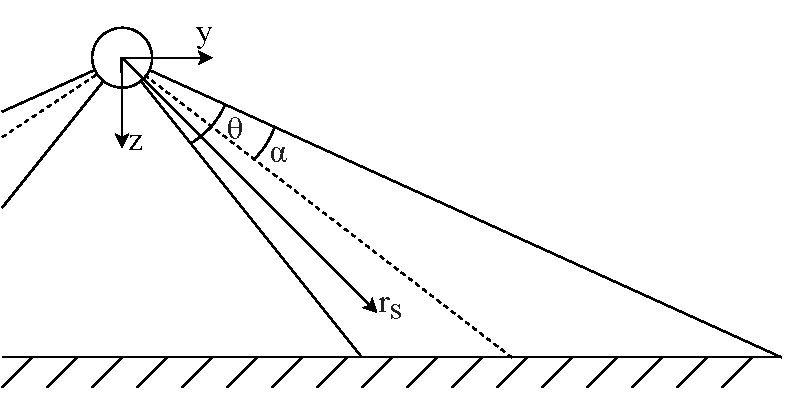
\includegraphics[trim=0cm 0cm 0cm 3.1cm, clip=true, width=0.7\textwidth]{figures/sss.drawio.pdf}
    \caption{Typical configuration of the side scan sonar.}
    \label{fig:sss}
\end{figure}

\begin{figure}[ht]
    \centering
    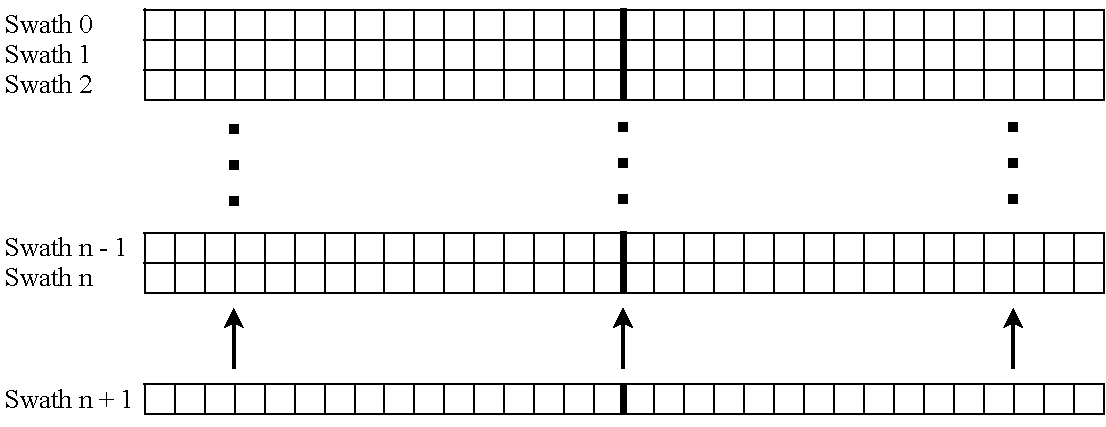
\includegraphics[width=0.8\textwidth]{figures/stacking_of_sonar_image.drawio.pdf}
    \caption{The figure shows how swaths are stacked together to form a sonar image.}
    \label{fig:stacking_of_sonar_image}
\end{figure}

\section{Data normalization and smoothing}

Cubic splines can be used to both normalize SSS data \cite{ReitanHogstad2022Side-ScanAutonomy} and to smooth the data to remove noise \cite{Al-Rawi2017LandmarkImages}. To normalize the SSS data, cubic spline regression estimates the underlying distribution of intensity values. For smoothing the SSS data, the cubic spline regression is used as the new smoothed data. The cubic smoothing spline, $f$, is 

\begin{equation}
    {f}(x) = \min_{f} p \sum_{i=1}^n |y_i-f(x_i)|^2 + (1-p) \int|D^2f(t)|^2dt,
    \label{eq:cubic_spline}
\end{equation}

where the first term is the error term and the second is the roughness measure,  where the integral is taken over the smallest interval containing all the entries of $x$. Further, $n$ is the number of data entries, $y_i$ sample $i$ of the data, $D^2f$ is the second derivate of $f$, and $p \in [0,1]$ is the smoothing parameter used to weigh between the error term and the roughness measure. 

For smoothing SSS data, each of the swaths is divided into a left and right swath, coming from the left and right transducer. The left and right parts of the swath are smoothed individually to form a cubic spline regression of the data, resulting in $\hat{I}(z) = f(z)$ for each bin, where $f$ is the smoothing cubic spline of the swath, found from \cref{eq:cubic_spline}.

Normalization, on the other hand, estimates the underlying distribution by cubic spline regression to normalize the data by

\begin{equation}
    \hat{I}(z) = \frac{I(z)}{f(z)},
    \label{eq:swath_norm}
\end{equation}

where $I(z)$ is the echo intensity at bin $z$, and again $f$ is the smoothing cubic spline of the swath, found from \cref{eq:cubic_spline}.

\section{Landmark detection}

Landmark detection is to detect interesting features, or in other words, landmarks, from data generated from observing the surroundings. For underwater applications, this can be translated to detect natural or artificial objects on the seafloor for SSS data. Due to SLAM for underwater vehicles being a challenging research topic \cite{Hidalgo2015ReviewTechniques}, the current research on landmark detection is not rich. A closely related research topic is the detection of mines on the seafloor, where the object also is to detect objects of interest on the seafloor \cite{Picard2016DetectionDimensionality}. In general, there are two main categories for detecting landmarks on the seafloor, either by classical methods, finding the echoes and/or shadows of the landmarks, or by using machine learning to detect the features. In recent years, using the rapidly evolving field of deep learning to do feature detection in sonar images has grown in popularity \cite{Wang2020ImageSonar, Zhou2022NonlinearFeatures}. However, the results generated from machine learning can be hard to explain and demands a lot of annotated data. Because of this, this report has chosen to focus on landmark detection using classical methods, and, therefore, machine learning for landmark detection will not be treated further.

Classical landmark detection methods for side scan sonar data exploit signal and image processing methods to find echoes and shadows in SSS data to detect landmarks. Classical methods can further be split into finding shadows and/or echoes in 1-dimensional swaths or 2-dimensional sonar images.

By doing peak detection, finding echoes and shadows in swaths is done in \cite{Al-Rawi2017LandmarkImages}. First, a smoothing by use of cubic splines is performed. Next, echoes are found by simple peak detection, whereas shadows are found by inverting the signal and performing peak detection. The first peak for shadows and echoes is removed since it represents the blind zone and the first bottom return (FBR), respectively, and not a landmark. A threshold based on the width and prominence of the peaks is used to remove insignificant peaks and find the landmarks.  

Landmark detection on 2D sonar images is the most common approach when doing classical landmark detection \cite{Wang2017UnderwaterSonar, Siantidis2016SideVehicles, Yuan2016AnNavigation, Leblond2019SonarProject}. The general approach uses a threshold to segment the image, either chosen arbitrarily or found adaptively. Depending on the method, the image is segmented into background, shadows, and/or echoes. Further, the shadows and/or echo landmarks are filtered to find landmarks with specific properties. \cite{Leblond2019SonarProject} filters shadows based on their geometrical properties to find consistent landmarks. 

\section{Generating consistent landmarks}

Morphological operators can be utilized to ensure consistent landmarks \cite{Yuan2016AnNavigation}. Morphological operators are a well-known image-processing tool based on a structuring element that is slid over the image, one pixel at a time, to compute new pixel values \cite{Gonzalez2018DigitalProcessing}. \cref{fig:image_processing_basics} shows the three first steps of such a process. Here the structuring element is of size $3\times3$ with the anchor point at the center. To ensure that the resulting image has the same size as the original image, padding can be added around the image's border. The values in the padding pixels can be chosen depending on the application. For example, it can reflect the image, replicate its border or be a constant pixel value.  

\begin{figure}
    \centering
    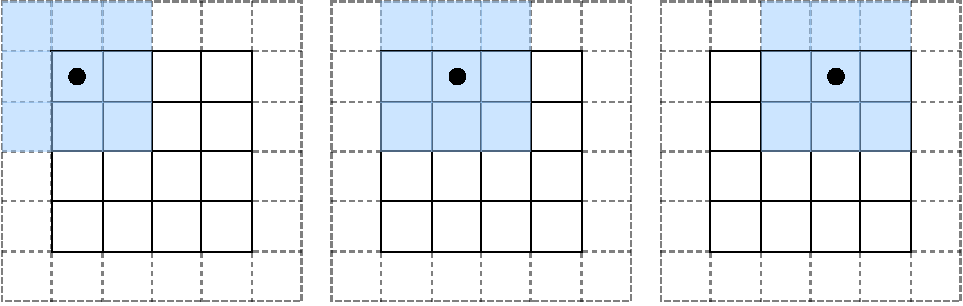
\includegraphics[width=0.8\textwidth]{figures/Image_processing_essentials.drawio.pdf}
    \caption{The image shows the three first steps (from left to right) of a general image processing method using a structuring element that is moved along the image to compute new pixel values. The black dot corresponds to the anchor point of the structuring element. The image is padded to get a new image of the same size as the original.}
    \label{fig:image_processing_basics}
\end{figure}

The four basic morphological operators are erosion, dilation, closing, and opening, where the two latter are a combination of the first operations. Both the image and the structuring element have binary values. Let $I_{SE}(x,y)$ be the extracted binary values from the part of the image covered by the structuring element, where $I_{SE}(x,y)$ has the same size as the structuring element, and let $S(x,y)$ be the structuring element of size $m \times n$. Then the erosion is defined as 

\begin{equation}
    \begin{split}
        I(a_x,a_y) = \prod_{i = 1}^m \prod_{j = 1}^n f(i,j) \\
        f(x,y) = 
        \begin{cases}
        I_{SE}(x,y) & S(x,y) \neq 0 \\
        1 & otherwise
        \end{cases}
    \end{split}
    \label{eq:erosion}
\end{equation}

and the dilation as

\begin{equation}
    I(a_x,a_y) = min(1, \sum_{i = 1}^m \sum_{j = 1}^n I_{SE}(i,j) \; S(i,j)).
    \label{eq:dialation}
\end{equation}

where $I(a_x,a_y)$ is the resulting intensity at the anchor point of the structuring element. The effect of an erosion operation is that all objects are shrunk, and small objects are removed. On the other hand, dilation results in all objects being thickened and holes in objects being filled. The effects of eliminating small objects and filling holes help generate consistent landmarks. However, the side effect of shrinking and thickening objects are unwanted. A dilation and erosion operation is combined to revert the side effects, and the new operations are called opening and closing. An opening operation is an erosion followed by a dilation, effectively removing small objects from the image. Closing is a dilation followed by erosion, eliminating holes in the image. 

\chapter{Method}

This chapter will present the two landmark detector methods and their inner workings. In addition, a novel quality indicator for SSS data is presented.

\section{Quality indicator for side scan sonar data}

The novel quality indicator calculates the overlapping of consecutive swaths, considering the ground range at maximum sensor opening. The motivation behind the quality indicator is to easily be able to pick out the areas of a sonar image where the turning of the AUV affects the quality of the data, causing anomalies in the sonar image. \cref{fig:r_eff} shows the SSS configuration, where $\theta$ is the mounting angle for the transducers from the horizontal line, $\alpha$ is the sensor opening, $h$ is the AUVs altitude above the seafloor, and $r_{g, max}$ is the maximum ground range. Because of varying altitudes, $h$, the maximum sonar ground range does not represent the range where we expect to find meaningful data. The \textit{effective ground range}, $r_{g, eff}$, on the other side, is a better representation and is given by

\begin{equation}
    r_{g,eff} = \frac{h}{tan(\theta - \frac{\alpha}{2})}.
    \label{eq:r_g_eff}
\end{equation}

\begin{figure}
    \centering
    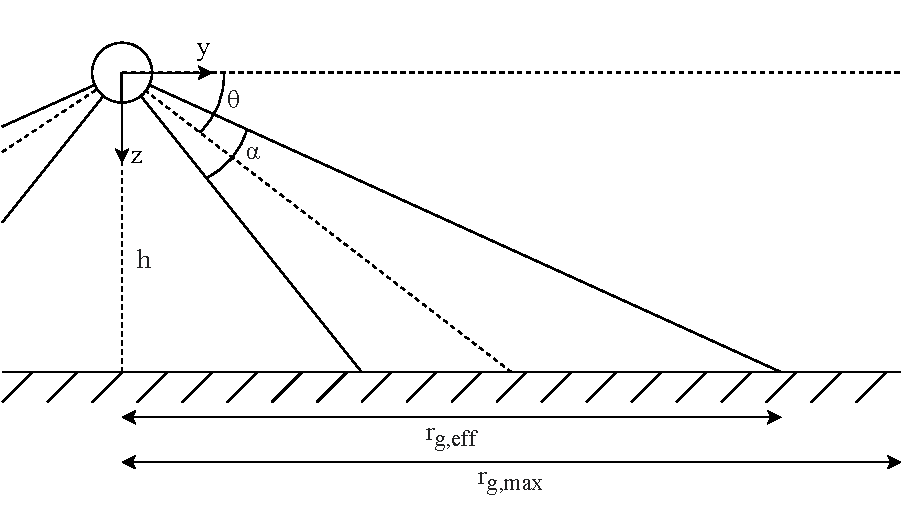
\includegraphics[width=0.8\textwidth]{figures/r_eff.drawio.pdf}
    \caption{Side scan sonar where $r_{eff}$, used in calculating the quality indicator, is shown.}
    \label{fig:r_eff}
\end{figure}

\cref{fig:quality_ind} show the AUV at two consecutive timesteps, where $\Delta \psi$ is the absolute change in heading between the two timesteps (i.e., positive for both left and right turn), $\Delta d$ the distance traveled in the xy-plane between the two timesteps and $r_{g, max}$ and $r_{g, eff}$ are the maximum and effective ground range, respectively. The distance between the AUV and the point on the swath where the next swath is crossing is $l$ (could be at infinity in case of $\Delta \psi = 0$) and is given by

\begin{equation}
    l = \frac{\Delta d}{tan(\Delta \psi)}.
    \label{eq:l_qi}
\end{equation}

Using the above results, the following quality indicator is proposed

\begin{equation}
    q = \frac{1}{2}[tanh( \,k\, [\frac{l}{r_{g, eff}} - \frac{1}{2}]) + 1]
\end{equation}

where $k$ is a tuning parameter, set to $k = 6$, used to tune the sensitivity of the quality indicator. 

\begin{figure}
    \centering
    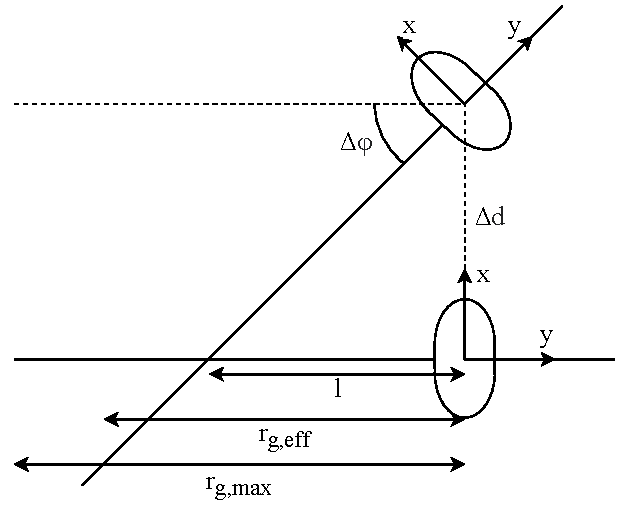
\includegraphics[width=0.55\textwidth]{figures/quality_ind.drawio.pdf}
    \caption{The figure shows an AUV for two consecutive timestamps, showing how the swaths can overlap due to the AUV turning.}
    \label{fig:quality_ind}
\end{figure}

\section{1D landmark detector using peak detection}

The 1D landmark detector, as in \cite{Al-Rawi2017LandmarkImages}, does peak detection in scan lines to find shadows and echoes and filter out non-significant echoes and shadows using a simple threshold. In this context, peak detection finds all local maxima in the swath. Landmarks are detected in one swath at a time, and peak detection is performed separately for the left and right parts of the swath. The first step for detecting meaningful peaks is to perform a smoothing of the swath, which is done by using a cubic spline. Next, the echoes are detected by detecting all peaks in the swath, and the shadows are detected by flipping the swath and detecting all peaks in the flipped swath. In addition to the position of all the peaks, the prominence and the width half-prominence are found. \cref{fig:1D_swath_w_landmarks} shows the result of detecting the echoes and shadows using peak detection. In addition, the peak of the FBR to the left swath is shown with its prominence and half-prominence width.
Further, all the shadows and echoes are filtered to detect landmarks. The first step is to remove the echo from the FBR and the shadow from the blind zone, as these are not generated from landmarks. These are the two most significant echoes and shadows in \cref{fig:1D_swath_w_landmarks}. Next, all echoes and shadows are filtered by a simple threshold given by

\begin{equation}
    E = \frac{2 width}{prominence}.
    \label{eq:1D_thres}
\end{equation}

\begin{figure}
    \centering
    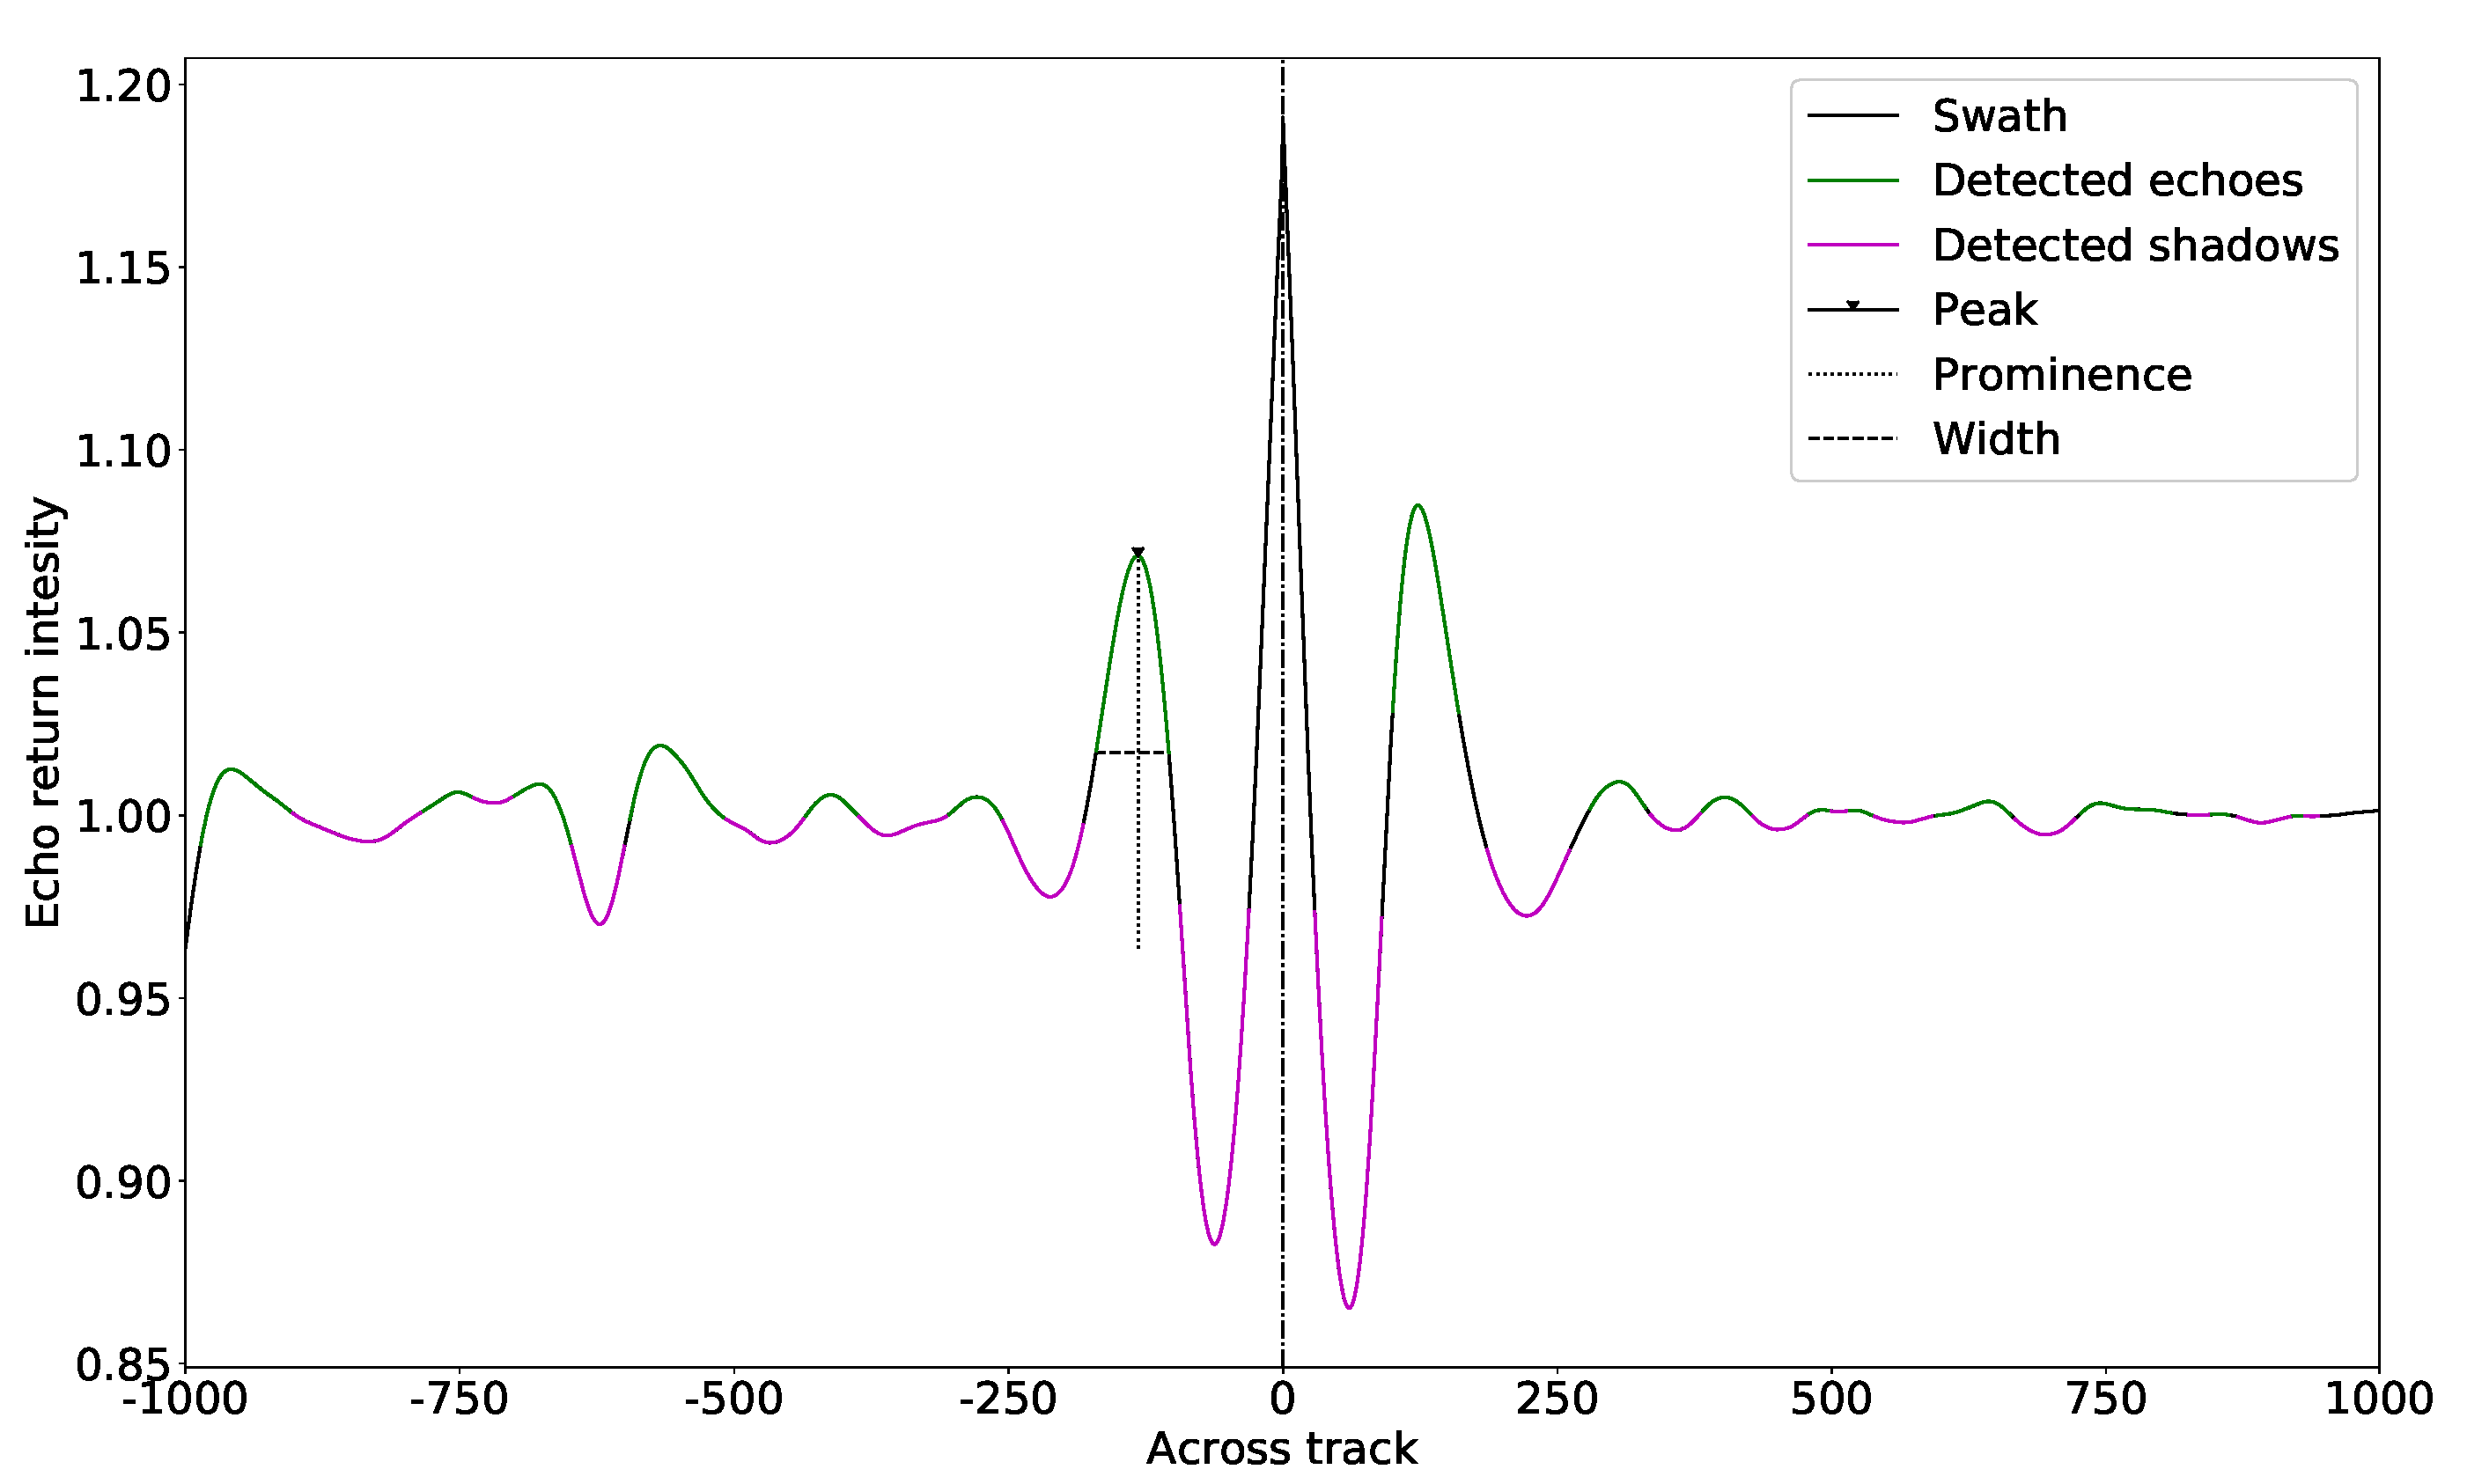
\includegraphics[width=0.8\textwidth]{figures/1D_swath_w_landmarks.eps}
    \caption{Normalized swath with all detected echoes and landmarks before filtering. The peak at the first bottom return for the left swath with its prominence and half-prominence width is also shown.}
    \label{fig:1D_swath_w_landmarks}
\end{figure}

In \cite{Al-Rawi2017LandmarkImages}, un-normalized SSS data is used, but the use of normalized data is suggested as an improvement. This report will present the result of performing landmark detection on normalized and unnormalized data. In addition, further improvements are suggested by applying morphological operators to remove thin landmarks and improve consistency. In the works of this report, a combination of a closing operation followed by an opening operation is tested on 2D binary images, constructed of shadows and echoes from the result of detecting landmarks in normalized data. 

\section{2D landmark detector using expert rules}

The 2D landmark detector, as in \cite{Leblond2019SonarProject}, finds shadows by intensity thresholding and uses a set of rules to filter out the shadows of the right size and shape. The first step is to perform an intensity thresholding on all the pixels to find shadows. The suggested intensity threshold is

\begin{equation}
    t_i = \frac{\Bar{I(x,y)}}{2},
    \label{eq:orginal_int_thres}
\end{equation}

where $\Bar{I(x,y)}$ is the average pixel intensity in the sonar image. However, this threshold produced close to no shadows from the data, so a new intensity threshold is suggested

\begin{equation}
    t_i = [\Bar{I(x,y)} - I(x,y)_{min}] k_i + I(x,y)_{min},
\end{equation}

where $I(x,y)_{min}$ is the average over the $100$ pixels with the lowest intensity, which increases robustness. Here, $k_i$ is a tuning parameter ranging from $0$ to $1$. Using the result from the intensity thresholding, a series of filtering rules are applied to filter out shadows. First, the shadows get filtered based on how many swaths they span over, where both minimum and maximum height filtering is applied. Second, filtering based on the area of the shadows in $pixels^2$ is applied. To account for how the grazing angle affects the shadows, the area is corrected by

\begin{equation}
    A_{corr} = A_s \frac{r_{ob,min}}{r_{ob}},
    \label{eq:corrected_area}
\end{equation}

where $r_{ob, min}$ is a reference object ground range that is tuneable, $r_{ob}$ is the ground range to the object, and $A_s$ is the area of the shadow in $pixels^2$. The last step is to filter the shadows based on how much of the bounding box that surrounds them that are filled, where the fraction of the filled area is given by

\begin{equation}
    \frac{A_s}{A_{bb}},
    \label{eq:fill_rate_bb}
\end{equation}

where $A_{bb}$ is the area of the bounding box surrounding the shadow. The bounding box's fill rate is compared to the fill rate threshold, $t_{fr}$. In addition to the proposed rules and tuning parameters, this report adds a closing operation to generate consistent landmarks. The structuring element (SE) is restricted to be quadratic, giving a new tuning parameter, $s_c$, for the size of the quadratic structuring element used for the closing operation. \cref{tab:2D_tuning_rules} summarises all tunable parameters and corresponding filtering rules. 

\begin{table}
    \begin{center}
    \caption{The table shows all the tunable parameters for the 2D landmark detector and the corresponding filtering rules applied.}
    \begin{tabular}{ll}
        \hline
        \textbf{Tunable parameter} & \textbf{Filtering rule}                            \\ \hline
        $k_i$             & $I(x,y) < (\Bar{I(x,y)} - I(x,y)_{min}) k_i + I(x,y)_{min}$ \\ 
        $s_c$             & Morphological closing on the shadows with SE of size $k_c$  \\ 
        $n_{swaths,min}$  & $n_{swaths} > n_{swaths,min}$                               \\ 
        $n_{swaths,max}$  & $n_{swaths} < n_{swaths,max}$                               \\ 
        $r_{ob,min}$      & $A_{corr} = A_s\frac{r_{ob,min}}{r_{ob}}$                   \\ 
        $A_{min}$         & $A_{corr} > A_{min}$                                        \\ 
        $t_{fr}$          & $\frac{A_s}{A_{bb}} > t_{fr}$                               \\ 
        \hline
    \end{tabular}
    \end{center}
    \label{tab:2D_tuning_rules}
\end{table}

\section{Qualitative comparison}

This report makes a qualitative comparison of the landmark detectors' results to compare them against each other. To make a meaningful comparison, some grounds for comparison must be set. First and foremost, an understanding of what part of a sonar image is considered a landmark and what is just considered background is needed. Next, an understanding of what makes up consistent landmarks is also essential. Lastly, some grounds for comparing the tuning process have to be defined. 

To compare the methods, understanding what parts of the sonar image are actual landmarks and what properties are consistent with a landmark is needed. Firstly, a division into echo and shadow landmarks has to be done. Echoes are typically generated by objects standing out from the seafloor, reflecting more sound and generating a more significant echo intensity in the sonar image. On the other hand, shadows are generated by occlusion, either by objects on the seafloor or simply by holes at the seafloor, and give dark areas in the sonar image. In the context of SLAM, landmarks that are re-detectable with different gracing angles and heading angles are of interest, and this should be the primary objective. However, it is not trivial to point out the properties such landmarks will have. 

\cref{fig:object_shadow} shows the same object being observed with two different gracing angles, $\theta_{s,1}$ and $\theta_{s,2}$. The shadow sizes and the grey unknown areas are inverse-proportional to the gracing angle. As the grey areas are unobserved, the backside of the landmark is unknown, and there could even be a second, smaller landmark behind the detected landmark. Since the backside is unknown, it is hard to make assumptions about the echo of the landmark observed with a different heading angle. However, inferring this to how the shadow appears is easier since the front is known. In that sense, shadow landmarks are preferred over echo landmarks. Further, small landmarks are unwanted because they can easily be occluded or mistaken by noise. Large landmarks are also unwanted. This is because they might be only partially observed in one situation and then fully observed in the next, making data association hard. 

\begin{figure}
    \centering
    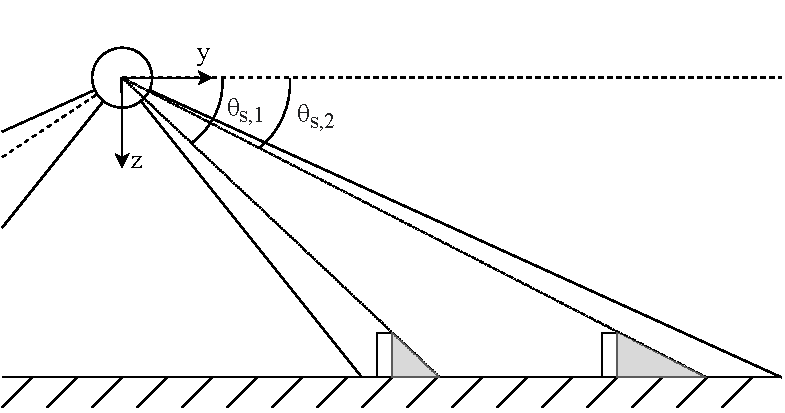
\includegraphics[width=0.7\textwidth]{figures/object_shadow.drawio.pdf}
    \caption{The figure shows how the same object, observed with two different gracing angles, generates different-sized shadows and that both the grey unknown areas and the shadow sizes are inverse-proportional to the gracing angle.}
    \label{fig:object_shadow}
\end{figure}

Landmark consistency is an essential qualitative measure and tells to what extent a landmark detection method can detect a landmark as one coherent landmark or several minor landmarks. The opposite is when what appears as one consistent landmark in the sonar image is either only detected partially or as several minor landmarks. The problem with partially detected or split landmarks is that small changes in how the landmark is observed can result in a landmark with a widely different form or size being detected. This, again, can lead to problems for the data association. 

Another vital measure when comparing landmark detection methods is how sensitive, complex, and intuitive the detector tuning is. Sensitivity is vital because if a method has a significant sensitivity, small changes in the operating conditions can significantly change performance. On the other hand, if the method has an acceptable performance over a wide range of parameters, it is more likely that the same is evident over a wide range of operating conditions. Next, the complexity of the tuning says something about how difficult it is to obtain good results and how interconnected the different parameters are in each other. Suppose the parameters do not have a great deal of interconnection. In that case, it is possible to tune one parameter at a time sequentially and end up with acceptable performance. In the opposite case, tuning one parameter will significantly influence the other parameters' effect on the performance, making it more difficult to obtain acceptable performance. Hence, the tuning is more complex. Last, how intuitive a tuning process is, is tightly related to the interpretation of the tuning parameters. If the parameters are only arbitrary sizes, their effect on the performance is generally less likely to be intuitive. On the other hand, the tuning can be said to be more intuitive if there is a direct relation between the parameters and the effect they have on the performance.     

\chapter{Results}

This chapter will present results from testing the landmark detector methods and the quality indicator on SSS data. The data was acquired in the Trondheims fjord by \textit{AURLab} using their vehicle \textit{LAUV Fridtjof} \cite{LAUVNTNU}. \cref{fig:neptus_screenshot} shows a map of parts of the Trondheim fjord and marks where the data was acquired. Further, the data was divided into a training and a test dataset of $4890$ and $3000$ swaths, respectively. The training dataset was used to tune the landmark detectors, and the test set was used to evaluate the performance. 

\begin{figure} [h]% order of priority: h here, t top, b bottom, p page
  \centering
  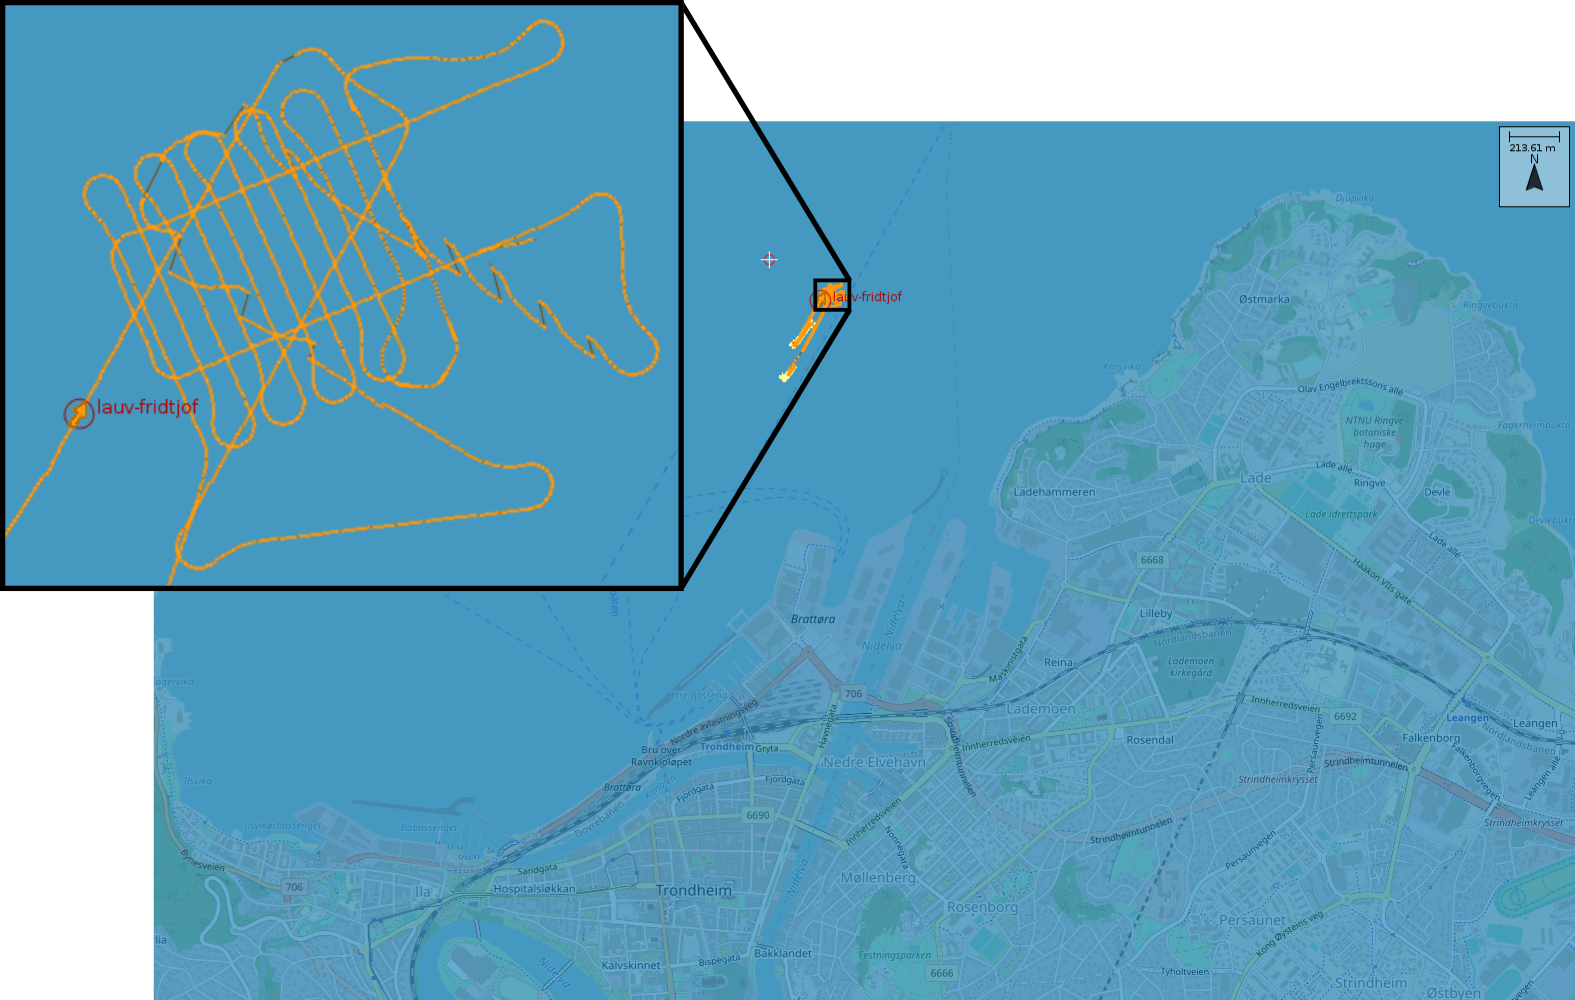
\includegraphics[width=0.9\textwidth]{figures/hercules_data.png}
  \caption{Map showing part of the Trondheim fjord and where the data in this report was acquired.}
  \label{fig:neptus_screenshot}
\end{figure}

\cref{fig:path_sonar_colorbars} shows the normalized trainingdata. On the right is the path of the AUV shown, and in addition, is the distance traveled in the xy-plane shown along the path. Since the AUV is assumed to have an approximately constant altitude during the survey, altitude data is omitted. The same distance traveled is shown on the right in the sonar image. As the speed of the AUV changes throughout the data, so will the scaling of the distance traveled; hence, the ticks shown can be used to give some sense of the distances in the path and the sonar image but can not be used accurately to infer the distance traveled between the plots. The swath numbers on the left side start to count from $0$. They, on the other hand, scale linearly but do not have any relation to the sizes on the seafloor. On the x-axis are the bin numbers displayed, where the left part of the swath span from $0$ to $-1000$ and the right part from $0$ to $1000$. Since the mapping from bin numbers to seafloor metrics vary with altitude along the path, it is non-trivial to present in an image like this; therefore, only the bin numbers are displayed. Investigating the sonar image closely, frequently occurring artificial lines going across the image can be observed. The same lines can be observed in \cref{fig:1D_raw_tuning_training}. The source of these lines is the transmission of the acoustic link between the AUV and a surface vessel. Further, the quality indicator is shown directly to the right of the sonar image in green-red-yellow colors, and its color scaling is shown on the far right of the figure. How it is calculated and its interpretation will be discussed below. On the right of the sonar image is the speed of the AVV in the xy-plane shown, and its color scaling is shown on the far right side. The color scaling of the quality indicator is the same throughout this report, but due to different speed ranges, the speed scaling differs between the training and test data. The color scaling for the test data is shown in \cref{fig:test_data}. 

\begin{figure}
    \centering
    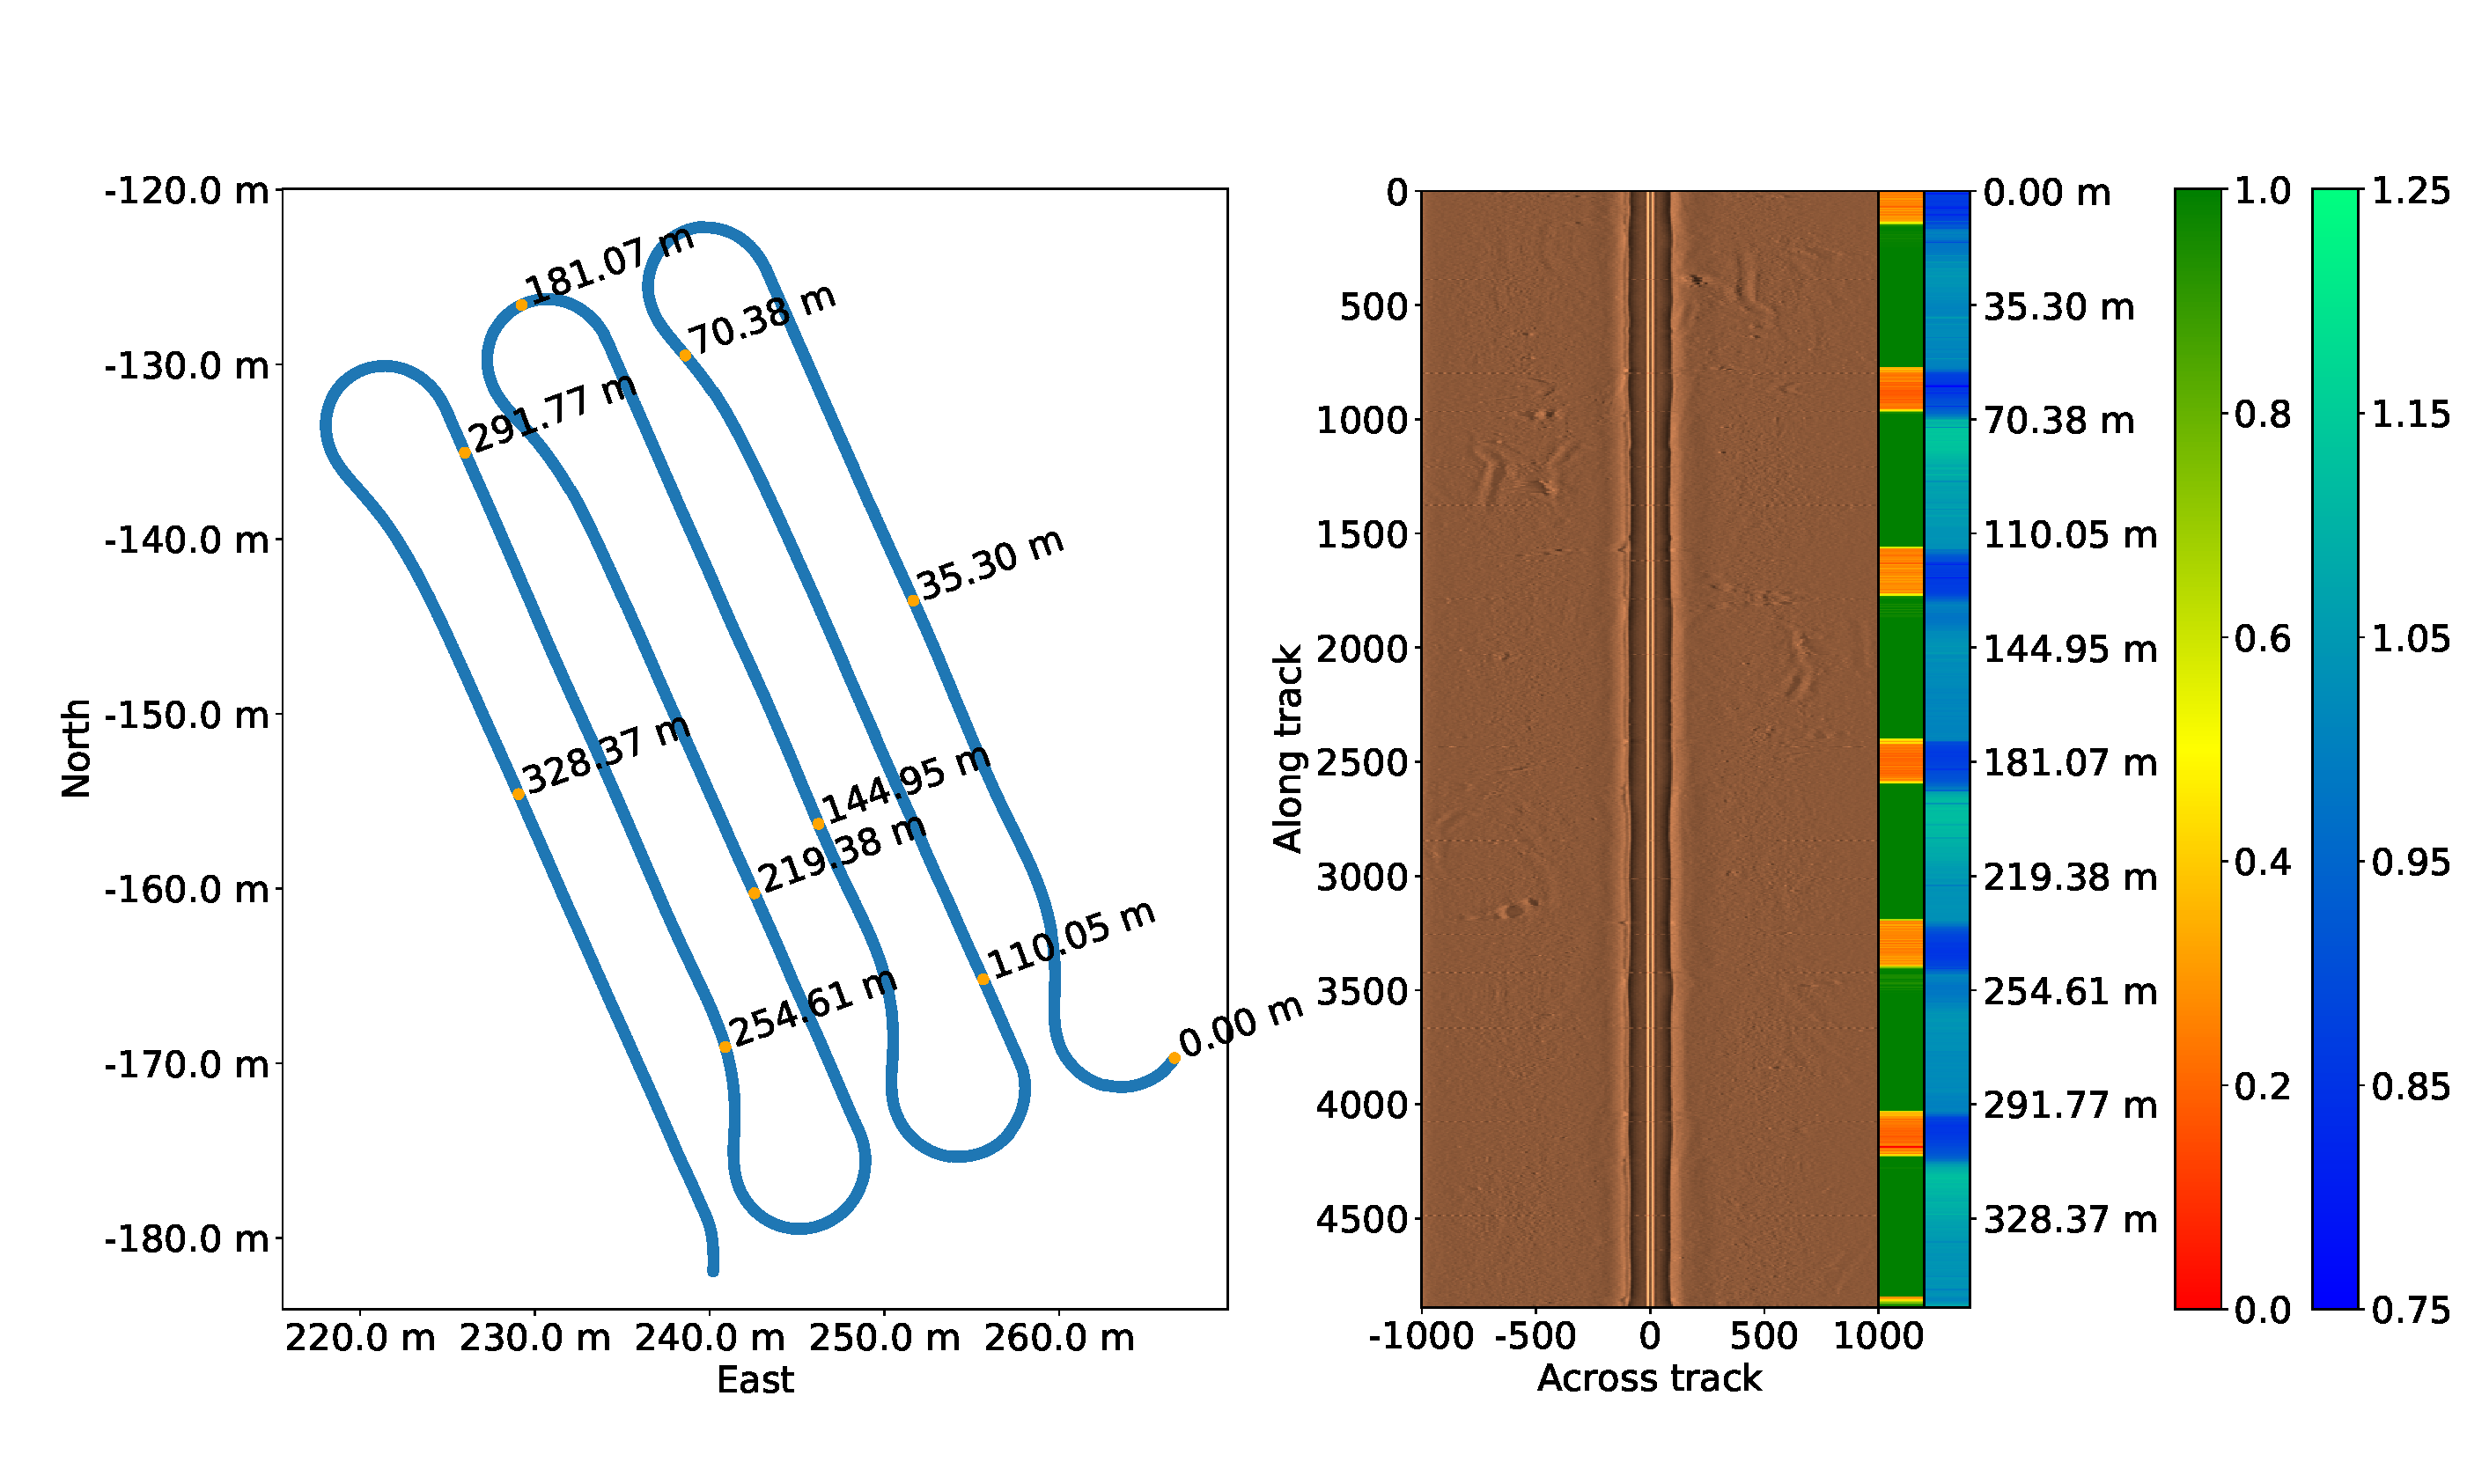
\includegraphics[trim=0cm 1.4cm 0cm 3.1cm, clip=true, width=1.0\textwidth]{figures/path_sonar_colorbars_training.eps}
    \caption{\textbf{Left:} The traveled path of the AUV from the training data set. In addition, the traveled distance is shown along the path. \textbf{Right:} The acquired normalized sonar image, from the training data with its corresponding quality indicator and speed in the xy-plane showed in direct relation, respectively. The color scaling of the quality indicator and speed used for all training data is shown on the far right.}
    \label{fig:path_sonar_colorbars}
\end{figure}

The main goal when tuning the landmark detector methods was to have as few possible false positives and the secondary to generate consistent landmarks. The number of false negatives was only slightly taken into consideration during tuning. This choice was made under the assumption that the geometrical properties of the landmarks will change depending on the gracing angle and azimuth angle they are observed under. Hence, will data association has a problematic starting point, to begin with, and providing it with several false positives will increase the probability that a wrong data association can be made. However, this choice is not trivial, and further work should investigate how the rate of false positives and false negatives affects the data association.

\section{Side scan sonar quality indicator}

The quality indicator is a measure that tries to say something about the quality of the SSS data, a measure that should be lower when turning due to overlapping swaths. \cref{fig:path_and_quality_ind} shows the result of testing the quality indicator on the training data. The top left side is a plot of the path of the AUV in the xy-plane. Further, the quality indicator is overlayed as the color of the path. As expected, the data quality decreases when turning due to swath overlapping. In addition, the traveled distance in the xy-plane is also shown along the path. The acquired sonar data traveling along the path is plotted on the right side, and the image's bars on the top right are the quality indicator and the speed of the AUV. The Dashed horizontal lines in the image are displayed to show approximately in which part of the image the poor quality occurs. At a traveled distance of around $60 m$, two banana-like shadows appear. These could typically be examples of the anomalies and degradation of quality experienced when turning during a sonar survey. The bottom part of the figure shows a zoomed-in part of the path. The black lines correspond to the effective ground range, the ground range for the maximum sensor opening, for two and two consecutive swaths. For $q = 1.0$, the swaths do not overlap, but for $q = 0.54$ and $q=0.24$, the swaths overlap at the blue "x"s. 

\begin{figure} % order of priority: h here, t top, b bottom, p page
  \centering
  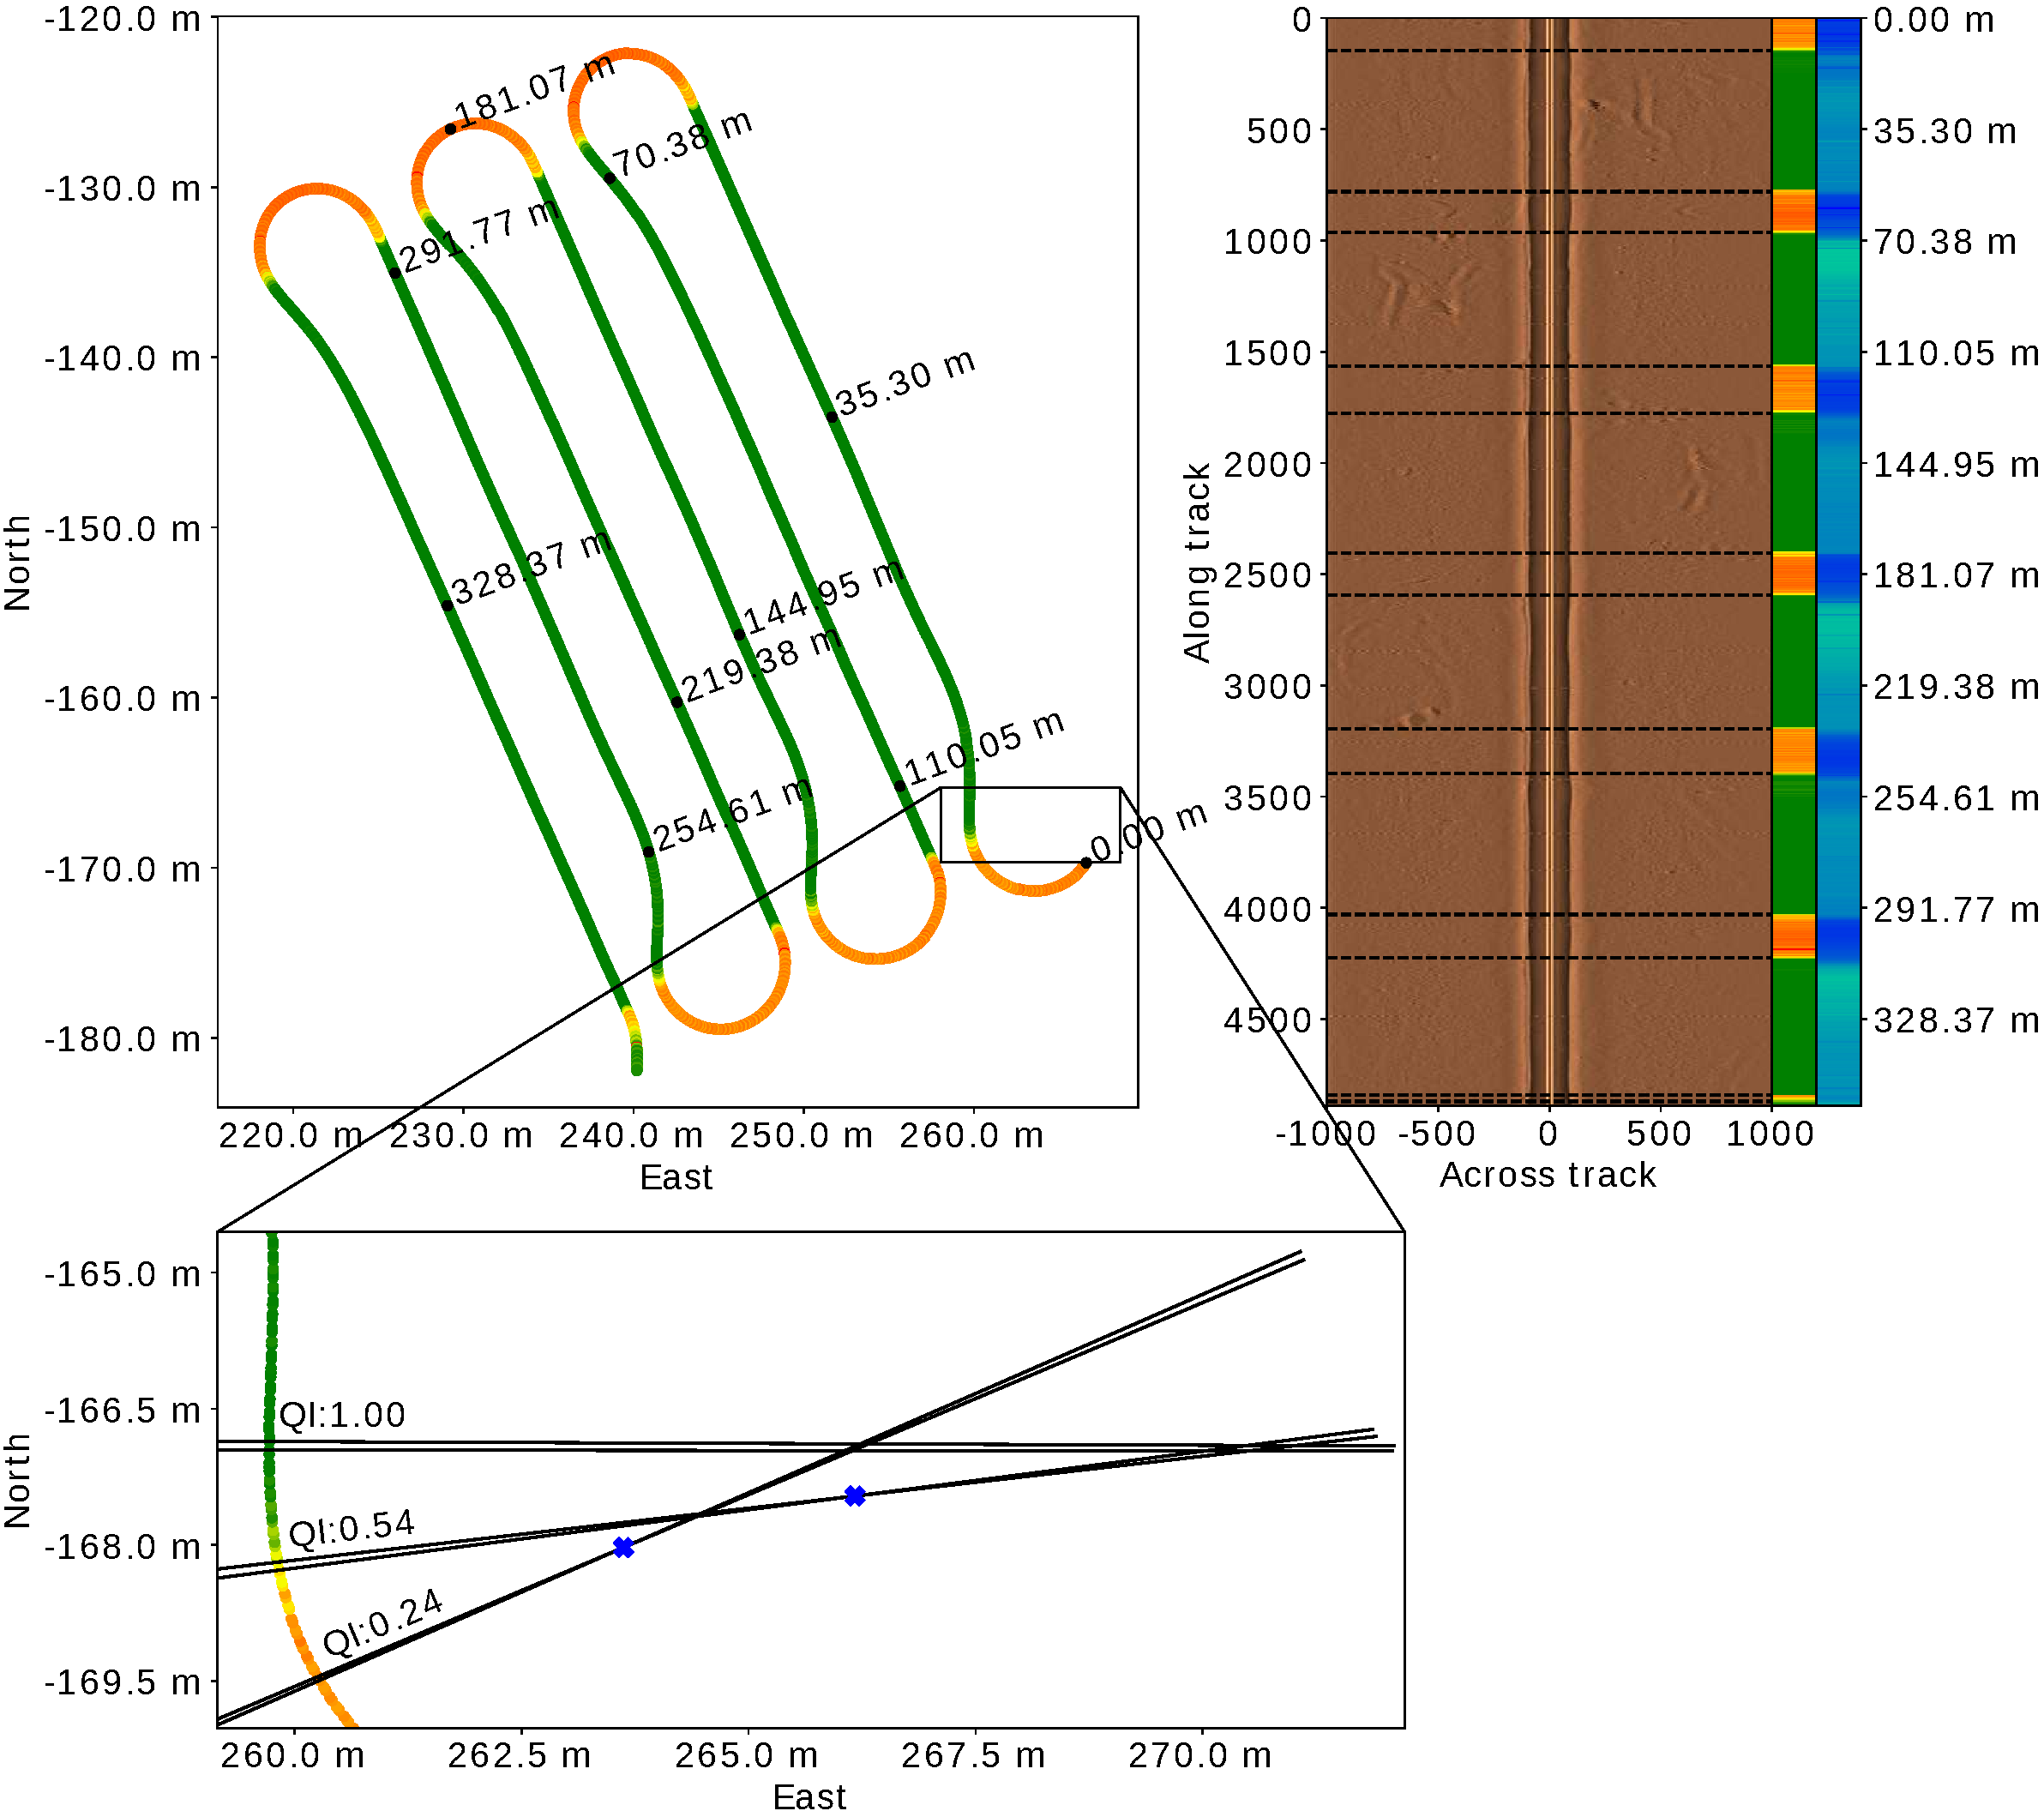
\includegraphics[trim=0cm 0cm 0cm 0cm, clip=true, width=0.9\textwidth]{figures/quality_indicator_and_path.pdf}
  \caption[Path with quality indicator overlayed]{\textbf{Top left:} The traveled path in the xy-plane of the AUV. The path's color corresponds to the quality indicator along the path, and the traveled distance is also shown. \textbf{Top right:} The right figure shows the sonar image acquired from moving along the path and the corresponding quality indicator. \textbf{Bottom:} A zoomed part of the path where the quality indicator is displayed as the color of the path, and the black lines correspond to the effective ground range for two and two consecutive swaths. The blue "x"s marks were two consecutive swath overlaps.}
  \label{fig:path_and_quality_ind}
\end{figure}

\section{1D Landmark Detector using Peak Detection}

The 1D landmark detector has two tuning parameters, the threshold filtering the shadows and echoes $E$ and the smoothing parameter $p$ for the cubic smoothing spline smoothing the data. \cref{fig:1D_raw_tuning_training} shows the results from tuning, with three different thresholds represented. The middle threshold of $E = 17$ was chosen. Even though there is not much difference between the different thresholds, there are some that make the selected threshold preferable over the other. For the threshold of $E = 16$, the clear shadow landmark around swath number $1300$ in the left swath loses some consistency compared to the chosen threshold of $E = 17$. For $E = 18$, two extra echo landmarks in the right swath around swath number $500$ were detected. The two extra detected landmarks are part of a larger landmark and are, together with the two connected shadow landmarks, an inconsistent detection of the landmark. A smoothing parameter of $p = \num{1e-5}$ was chosen to filter out enough noise not to get false positives. Further, some false positives are detected, but all of these are in connection to the acoustic communication with a surface vessel and are therefore not considered. 

% The 1D landmark detector has four tuning parameters, the threshold $t$, smoothing parameter $s$, and the kernel size of the quadratic kernels used for the opening and closing operators. \cref{fig:1D_norm_tuning_training} shows the results from tuning, with three different thresholds represented. The middle threshold of $t = 1550$ was chosen. Even though there is not much difference between the different thresholds, there are some that make the selected threshold preferable over the other. For the threshold of $t = 1500$, an echo landmark on the left swath at around swath number $3100$ is missing compared to the chosen threshold. For $t = 1600$, two extra landmarks in the left swath around swath number $1000$ and $1200$ are detected. The landmark at swath number $1000$ is a real landmark. However, the detected landmark around swath number $1200$ is only partially detected and is therefore unwanted. A smoothing parameter of $s = \num{1e-5}$ was chosen to filter out enough noise not to get false positives. As the figure shows, there are not a lot of false positives, but to a cost of filtering out a large fraction of the details. To further filter the landmarks, the quadratic kernel used for the closing operation was chosen with a size of $10^2$, and the size of the kernel for the opening operation was chosen as $15^2$, such that the detected landmarks are both consistent and that narrow landmarks are removed, respectively.  

\begin{figure}   % order of priority: h here, t top, b bottom, p page
  \centering
  \includegraphics[width=1.0\textwidth]{figures/1D_raw_tuning_training.eps}
  \caption[Results of tuning threshold of the 1D method]{Results from tuning the thresholds of the 1D method with three different thresholds on un-normalized data. The left image shows the unnormalized training data without any landmark detection. The three other images show the results using a threshold $E = 16$, $E = 17$, and $E = 18$. All images are smoothed with a smoothing parameter of $p = \num{1e-5}$. Shadow landmarks are shown in green and echo landmarks are in pink. The two bars on the right show the quality indicator and the vehicle's speed.}
  % Parameters used: smoothing e-5
  \label{fig:1D_raw_tuning_training}
\end{figure}

% \begin{figure}[ht]% order of priority: h here, t top, b bottom, p page
%      \centering
%     \begin{subfigure}[t]{0.3051\textwidth}
%          \centering
%          \includegraphics[trim=14cm 0cm 19.7cm 0cm, clip=true, width=\textwidth]{figures/1D_raw_result_training.eps}
%      \end{subfigure}
%      \hspace{0cm}
%      \begin{subfigure}[t]{0.2493\textwidth}
%          \centering
%          \includegraphics[trim=16.4cm 0cm 19.7cm 0cm, clip=true, width=\textwidth]{figures/1D_norm_result_training.eps}
%      \end{subfigure}
%      \hspace{0cm}
%      \begin{subfigure}[t]{0.3339\textwidth}
%          \centering
%          \includegraphics[trim=16.4cm 0cm 16.1cm 0cm, clip=true, width=\textwidth]{figures/1D_norm_morph_result_training.eps}
%      \end{subfigure}
%         \caption{\textbf{Left:} Result from tuning the 1D landmark detector on unnormalized training data with threshold $E = 17$. \textbf{Middle:} Result from tuning the 1D landmark detector on normalized training data with threshold $E = 1450$. \textbf{Right:} Results from tuning the 1D landmark detector on normalized training data with threshold $E = 1450$ and sizes for the quadratic structuring element of the closing and opening operation of $s_c = 10^2$ and $s_o = 15^2$, respectively. All results use a smoothing parameter of $p = \num{1e-5}$. The shadow landmarks are pink, and the echo landmarks are green.}
%         \label{fig:1D_tuning_results}
% \end{figure}

\begin{figure} [hb!]
    \centering
    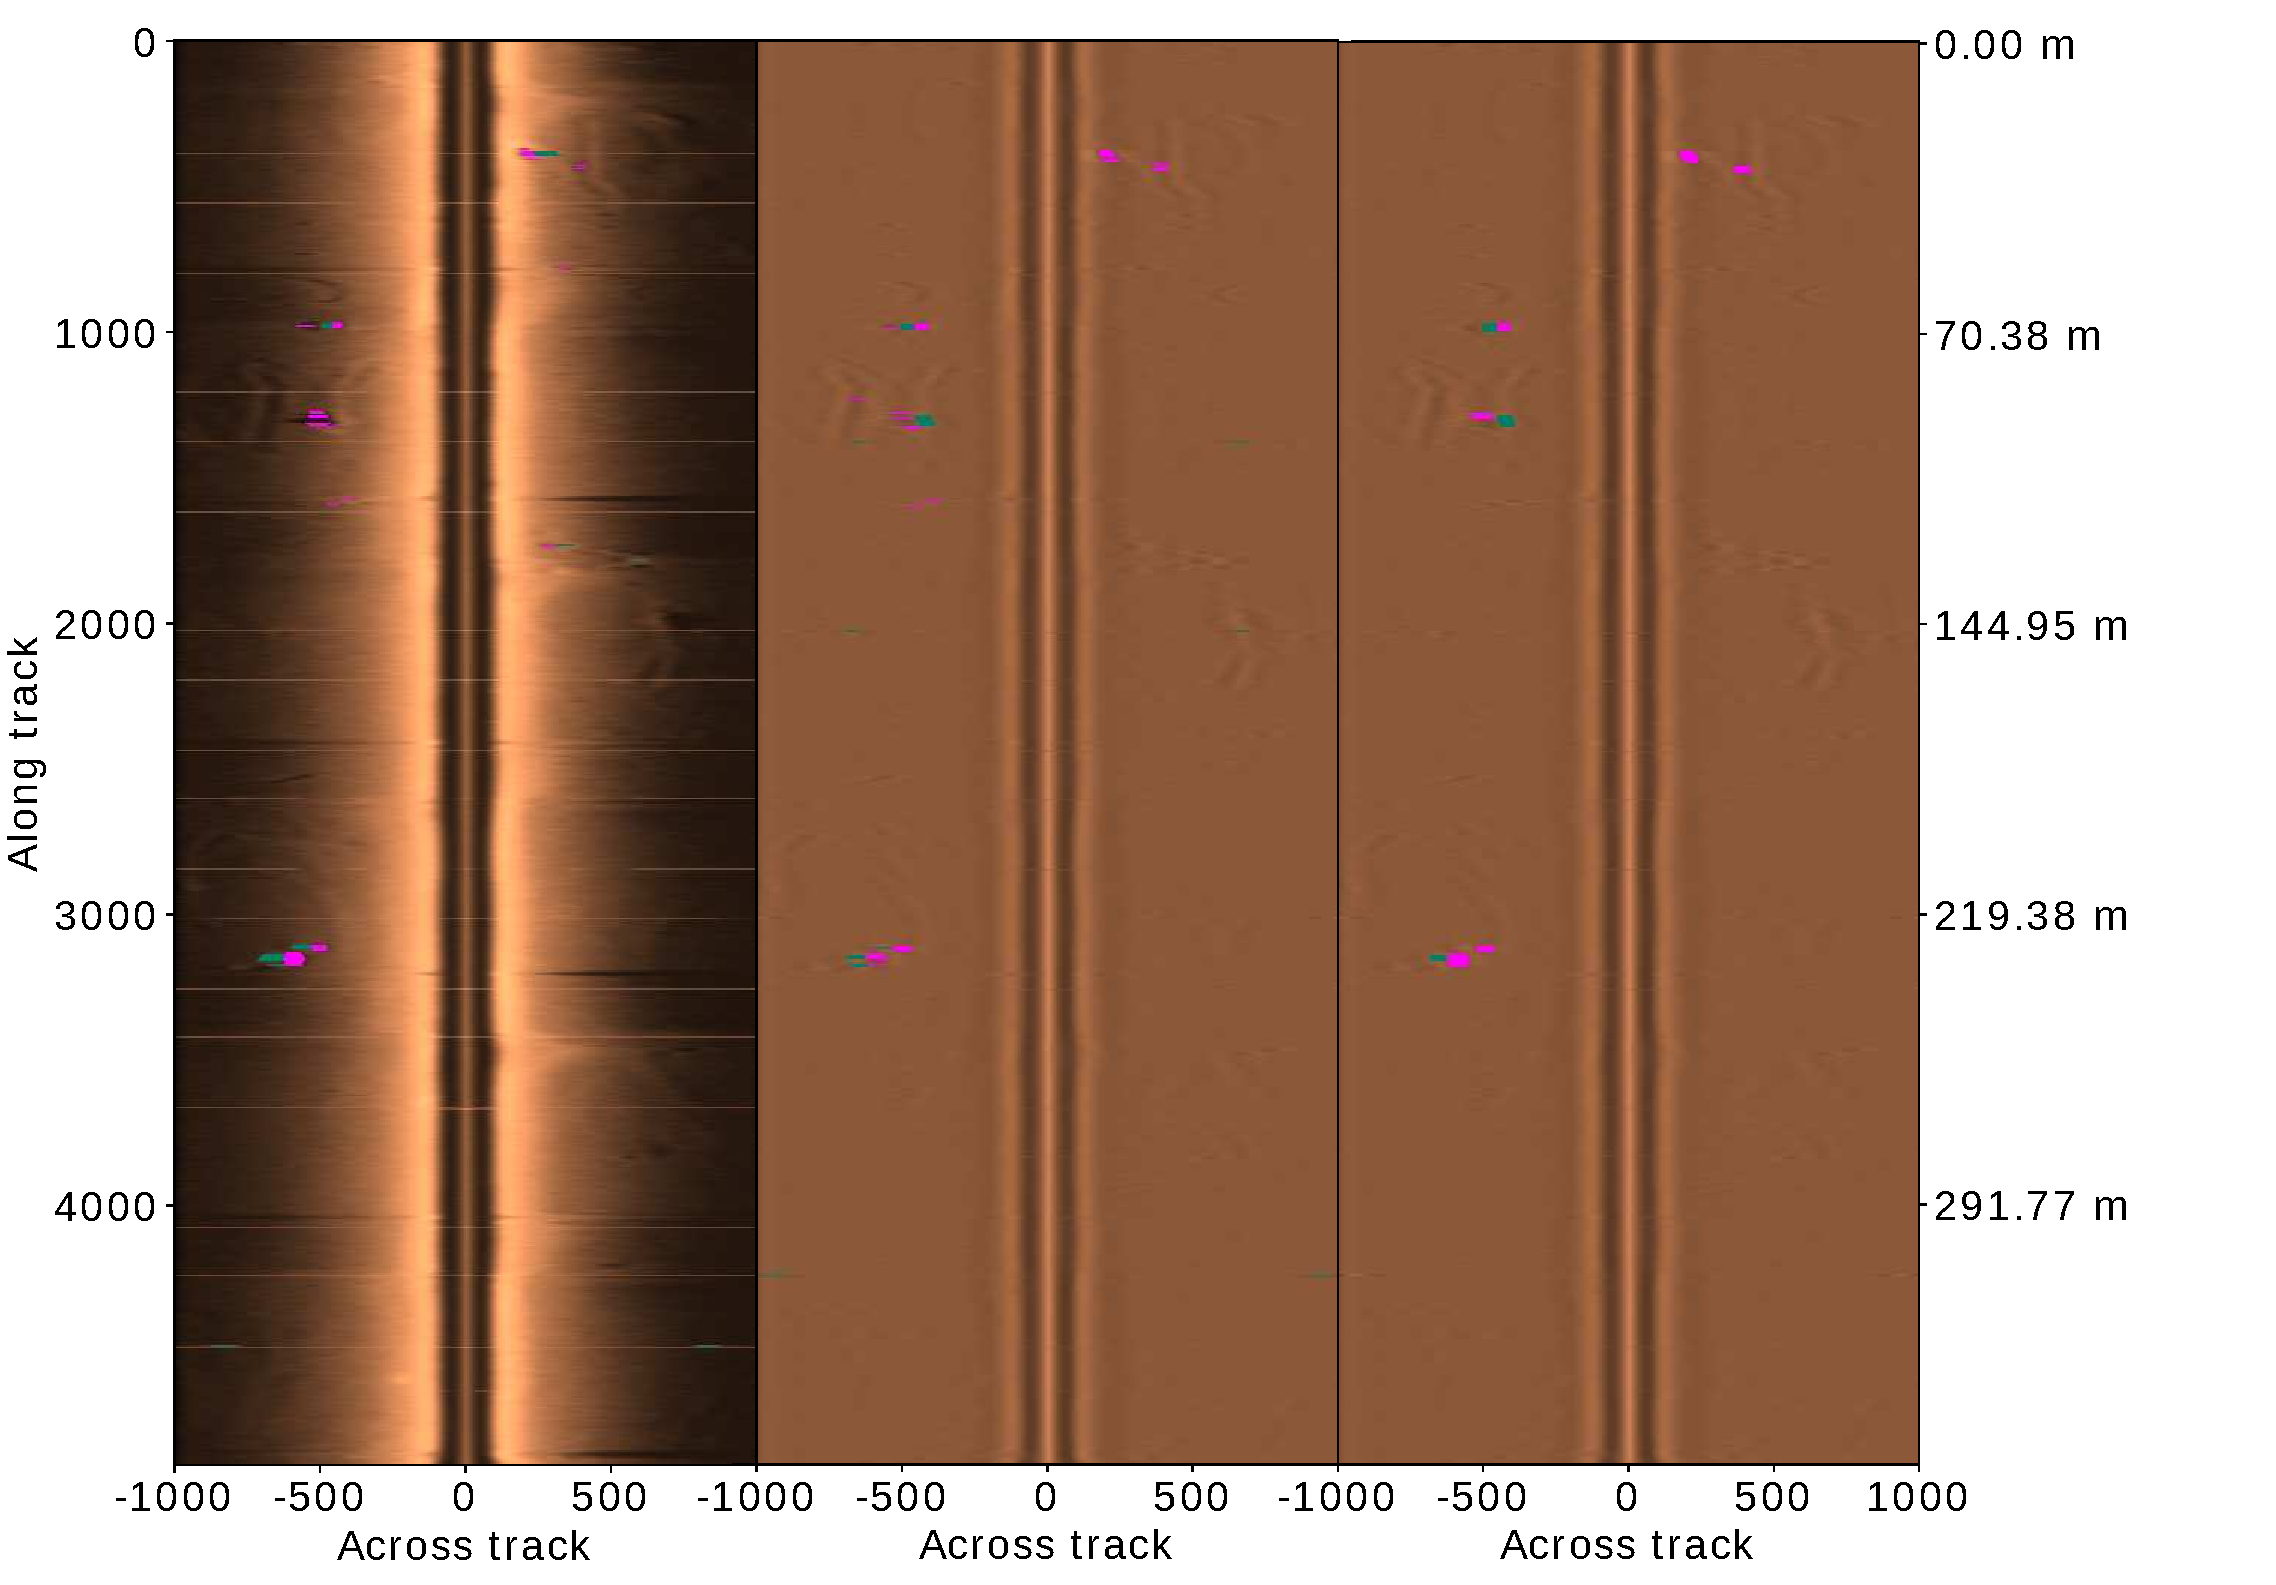
\includegraphics[trim=0cm 0cm 2.5cm 0cm, clip=true, width=0.8\textwidth]{figures/1D_result_training.pdf}
    \caption{\textbf{Left:} Result from tuning the 1D landmark detector on unnormalized training data with threshold $E = 17$. \textbf{Middle:} Result from tuning the 1D landmark detector on normalized training data with threshold $E = 1450$. \textbf{Right:} Results from tuning the 1D landmark detector on normalized training data with threshold $E = 1450$ and sizes for the quadratic structuring element of the closing and opening operation of $s_c = 10^2$ and $s_o = 15^2$, respectively. All results use a smoothing parameter of $p = \num{1e-5}$. The shadow landmarks are pink, and the echo landmarks are green.}
    \label{fig:1D_tuning_results}
\end{figure}

As suggested in \cite{Al-Rawi2017LandmarkImages}, using normalized data and morphological operators to filter out thin landmarks were tested, and \cref{fig:1D_tuning_results} shows the results. As discussed above, the left image results from using unnormalized training data with a threshold of $E = 17$. The middle image is the result of testing the method on normalized data. Using the same considerations as when tuning the 1D landmark detector on unnormalized data, a threshold of $E = 1450$ was found. Again, all false positives are considered to originate from acoustic communication. The false positives are all echo landmarks and appear in pairs, one on the left side and one on the right side of the swath, and can be found approximately in swath numbers $1300$, $2000$, and $4200$. In addition, a few landmarks are inconsistently detected. On the right side, the results of applying a closing operation followed by an opening operation with quadratic structuring elements of sizes $s_c = 10^2$ and $s_o = 15^2$ on the middle image are shown. The sizes of the structuring elements were found by testing different sizes and choosing the ones that generated results most aligned with the tuning goals. All false positives are removed, and the resulting landmarks are mostly consistent. Both the rightmost shadow landmark and the shadow landmark at around swath number $1200$ are part of a larger landmark and are inconsistently detected. All results used a smoothing parameter of $p = \num{1e-5}$. \cref{tab:1D_parameters} summarizes the parameters used. 

Comparing the results in \cref{fig:1D_tuning_results}, there is not much difference in the left and middle images using unnormalized and normalized data. However, as discussed in \cref{sec:disc_1D_landmark_detector}, normalized data is preferred over unnormalized data. Using morphological operators on normalized data gives significantly better results and is therefore chosen to compare against the 2D landmark detector.

\begin{table} [h!]
    \caption{Resulting parameters from tuning the 1D landmark detector on unnormalized and normalized training data.}
    \centering
    \begin{tabular}{cccc}
        \hline
        \textbf{Tunable parameter} & \textbf{Unnormalized} & \textbf{Normalized} & \textbf{Normalized with morph. operators} \\ \hline
        $E$                        & $17$                  & $1450$              & $1450$                                    \\
        $p$                        & $\num{1e-5}$          & $\num{1e-5}$        & $\num{1e-5}$                              \\
        $s_c$                      & $-$                   & $-$                 & $10^2$                                    \\
        $s_o$                      & $-$                   & $-$                 & $15^2$                                    \\ \hline
    \end{tabular}
    \label{tab:1D_parameters}
\end{table}

\section{2D Landmark Detector using Expert Rules}

The 2D landmark detector has a total of six parameters to tune. The parameter $r_{ob min}$ was set to $3 m $, as in \cite{Leblond2019SonarProject}. \cref{fig:2D_tuning_intensity_thres} shows the result from tuning the intensity threshold with three different intensity thresholds displayed. The intensity threshold of $k_i = 0.9$ was chosen. An intensity threshold of $k_i = 0.85$ results in less noise in the detected landmark candidates than the chosen threshold of $k_i = 0.9$. However, landmark candidates without a strong shadow are not detected consistently. Several large landmark candidates either have holes or are not consistently detected. An intensity threshold of $k_i = 0.95$ results in much more noise in the detected landmark candidates, which is unwanted. An intensity threshold of $k_i = 0.9$ produces consistent landmark candidates and an acceptable amount of noise. 

\begin{figure}[ht]  % order of priority: h here, t top, b bottom, p page
  \centering
  \includegraphics[trim=0cm 1.6cm 0cm 1.4cm, clip=true, width=0.9\textwidth]{figures/2D_tuning_threshold_training.eps}
  \caption[Results of tuning intensity threshold the 2D method]{Results from tuning the intensity thresholds of the 2D method with three different thresholds on normalized data. The left image shows the normalized training data without any thresholding. The three other images show the results using an intensity threshold $k_i = 0.85$, $k_i = 0.9$, and $k_i = 0.9$. All images are smoothed with a smoothing parameter of $p = \num{1e-2}$. Landmark candidates are shown in green. The two bars on the right show the quality indicator and the vehicle's speed.}
  \label{fig:2D_tuning_intensity_thres}
\end{figure}

\cref{fig:2d_tuning_paramaters_training} shows the results of tuning the last four parameters. The green landmark candidates are the landmarks filtered out in the corresponding step of the pipeline, and the pink landmarks are the kept landmarks. The leftmost image shows the sonar image. The second leftmost image results from filtering landmark candidates by how many swaths they are a part of, i.e., the height of the landmark candidate in the sonar image. The landmark candidates are generated by applying intensity thresholding on the sonar image. Large landmarks are chosen to be filtered out because it is more difficult to detect them consistently, and therefore a more conservative choice is made. The minor landmarks were also filtered out, resulting in $n_{swaths, min} = 50 \; swaths$ and $n_{swaths, max} = 150 \; swaths$. In addition, this step filters out much of the noise in the landmark candidates. The third image shows the result of applying the landmark area filtering. The parameter $A_{min} = 100 \;pixels^2$ was chosen to filter out the minor landmarks left from the height filtering. The fourth image shows the result of filtering out landmarks based on their fill rate of the rectangular bounding box encapsulating them. The fill rate limit was set to $t_{fr} = 0.3$ to filter out the thin and non-consistent landmarks. The last image shows the resulting landmarks.

\begin{figure} % order of priority: h here, t top, b bottom, p page
     \centering
    \begin{subfigure}[t]{0.975\textwidth}
        \centering
        \includegraphics[trim=0cm 3cm 0cm 2.8cm, clip=true, width=\textwidth]{figures/2D_tuning_parameters_training.eps}
        \caption{Results from tuning the 2D method on normalized data. An intensity threshold of $k_i = 0.9$ generates the landmark candidates used.}
        \label{fig:2d_tuning_paramaters_training}
     \end{subfigure}
     \hfill
     \begin{subfigure}[b]{0.975\textwidth}
        \includegraphics[trim=0cm 3cm 0cm 2.8cm, clip=true, width=1.0\textwidth]{figures/2D_filtered_tuning_parameters_training.eps}
        \caption{Results from tuning the 2D method on normalized data, using a closing operation to filter the landmark candidates. An intensity threshold of $k_i = 0.85$ followed by a closing operation with a quadratic SE of size $s_c = 10^2$ generates the landmark candidates used.}
        \label{fig:2d_tuning_paramaters_w_filtering_training}
     \end{subfigure}
        \caption{Results from tuning the 2D method on normalized data. In both figures, the left image shows the normalized training data without any detection. The four other images show the different steps in the pipeline, applying the different thresholds to the landmark candidates. The green landmark candidates are the landmarks filtered out in the corresponding step of the pipeline, and the pink landmarks are the kept landmarks. The two bars on the right show the quality indicator and the vehicle's speed.}
        %Both figures use $n_{swaths, min} = 50 \; swaths$, $n_{swaths, max} = 150 \; swaths$, $A_{min} = 100 \;pixels^2$, and $t_{fr} = 0.3$ and all images are smoothed with a smoothing parameter of $p = \num{1e-2}$. 
\end{figure}

Looking at the height filtering step in \cref{fig:2d_tuning_paramaters_training}, it is evident that two of the inconsistently detected landmarks (landmark number two and three from the top) are so because they are split by artifacts coming from acoustic communication. Drawing from the 1D landmark detector, a closing operation with a quadratic SE of size $s_c = 10^2$ is added between the intensity threshold step and the height filtering. \cref{fig:2d_tuning_paramaters_w_filtering_training} shows the tuning of the pipeline. Due to the more consistent landmark candidates, the amount of noise could be reduced by reducing the intensity threshold to $k_i = 0.85$. The other parameters were not changed. The two landmarks inconsistently detected earlier are not detected and rightly removed due to their height. Further, two new landmarks are detected. 

The resulting parameters are shown in \cref{tab:2D_parameters}. Comparing with and without morphological operators, using the closing operation helps with consistency; therefore, this is the preferred method for comparing with the 1D landmark detector. 

\begin{table} [ht]
    \caption{Resulting parameters from tuning the 2D landmark detector on normalized training data.}
    \centering
    \begin{tabular}{ccc}
        \hline
        \textbf{Tunable parameter} & \textbf{Normalized} & \textbf{Normalized with morph. operators} \\ \hline
        $k_i$                      & $0.9$               & $0.85$                                    \\
        $s_c$                      & $-$                 & $10^2$                                    \\
        $n_{swaths, min}$          & $50 \; swaths$      & $50 \; swaths$                            \\
        $n_{swaths, max}$          & $150\; swaths$      & $150 \; swaths$                           \\
        $r_{ob, min}$              & $3 \; m$            & $3 \; m$                                  \\ 
        $A_{min}$                  & $100 \; pixels^2$   & $100 \; pixels^2$                         \\
        $t_{fr}$                   & $0.3$               & $0.3$                                     \\ \hline
        
    \end{tabular}
    \label{tab:2D_parameters}
\end{table}

\newpage

\section{Landmark detection on test data}

Both landmark detector methods were run on the test dataset to evaluate the performance of the landmark detectors with the chosen tuning parameters. \cref{fig:test_data} shows the test data. The result from the 1D landmark detector is shown in \cref{fig:1D_norm_result_test}. No false positives are detected; however, several landmarks are only partially detected. It is also worth noting that only one echo landmark is detected. \cref{fig:2D_result_single_test} shows the result from the 2D landmark detector. The conservative tuning is evident in the result, as several large, thin landmarks at the top of the image are not detected. Further, the two thin landmarks that are detected are only partially detected. 

\begin{figure} [hb] % order of priority: h here, t top, b bottom, p page
     \centering
    \begin{subfigure}[t]{0.87\textwidth}
         \centering
         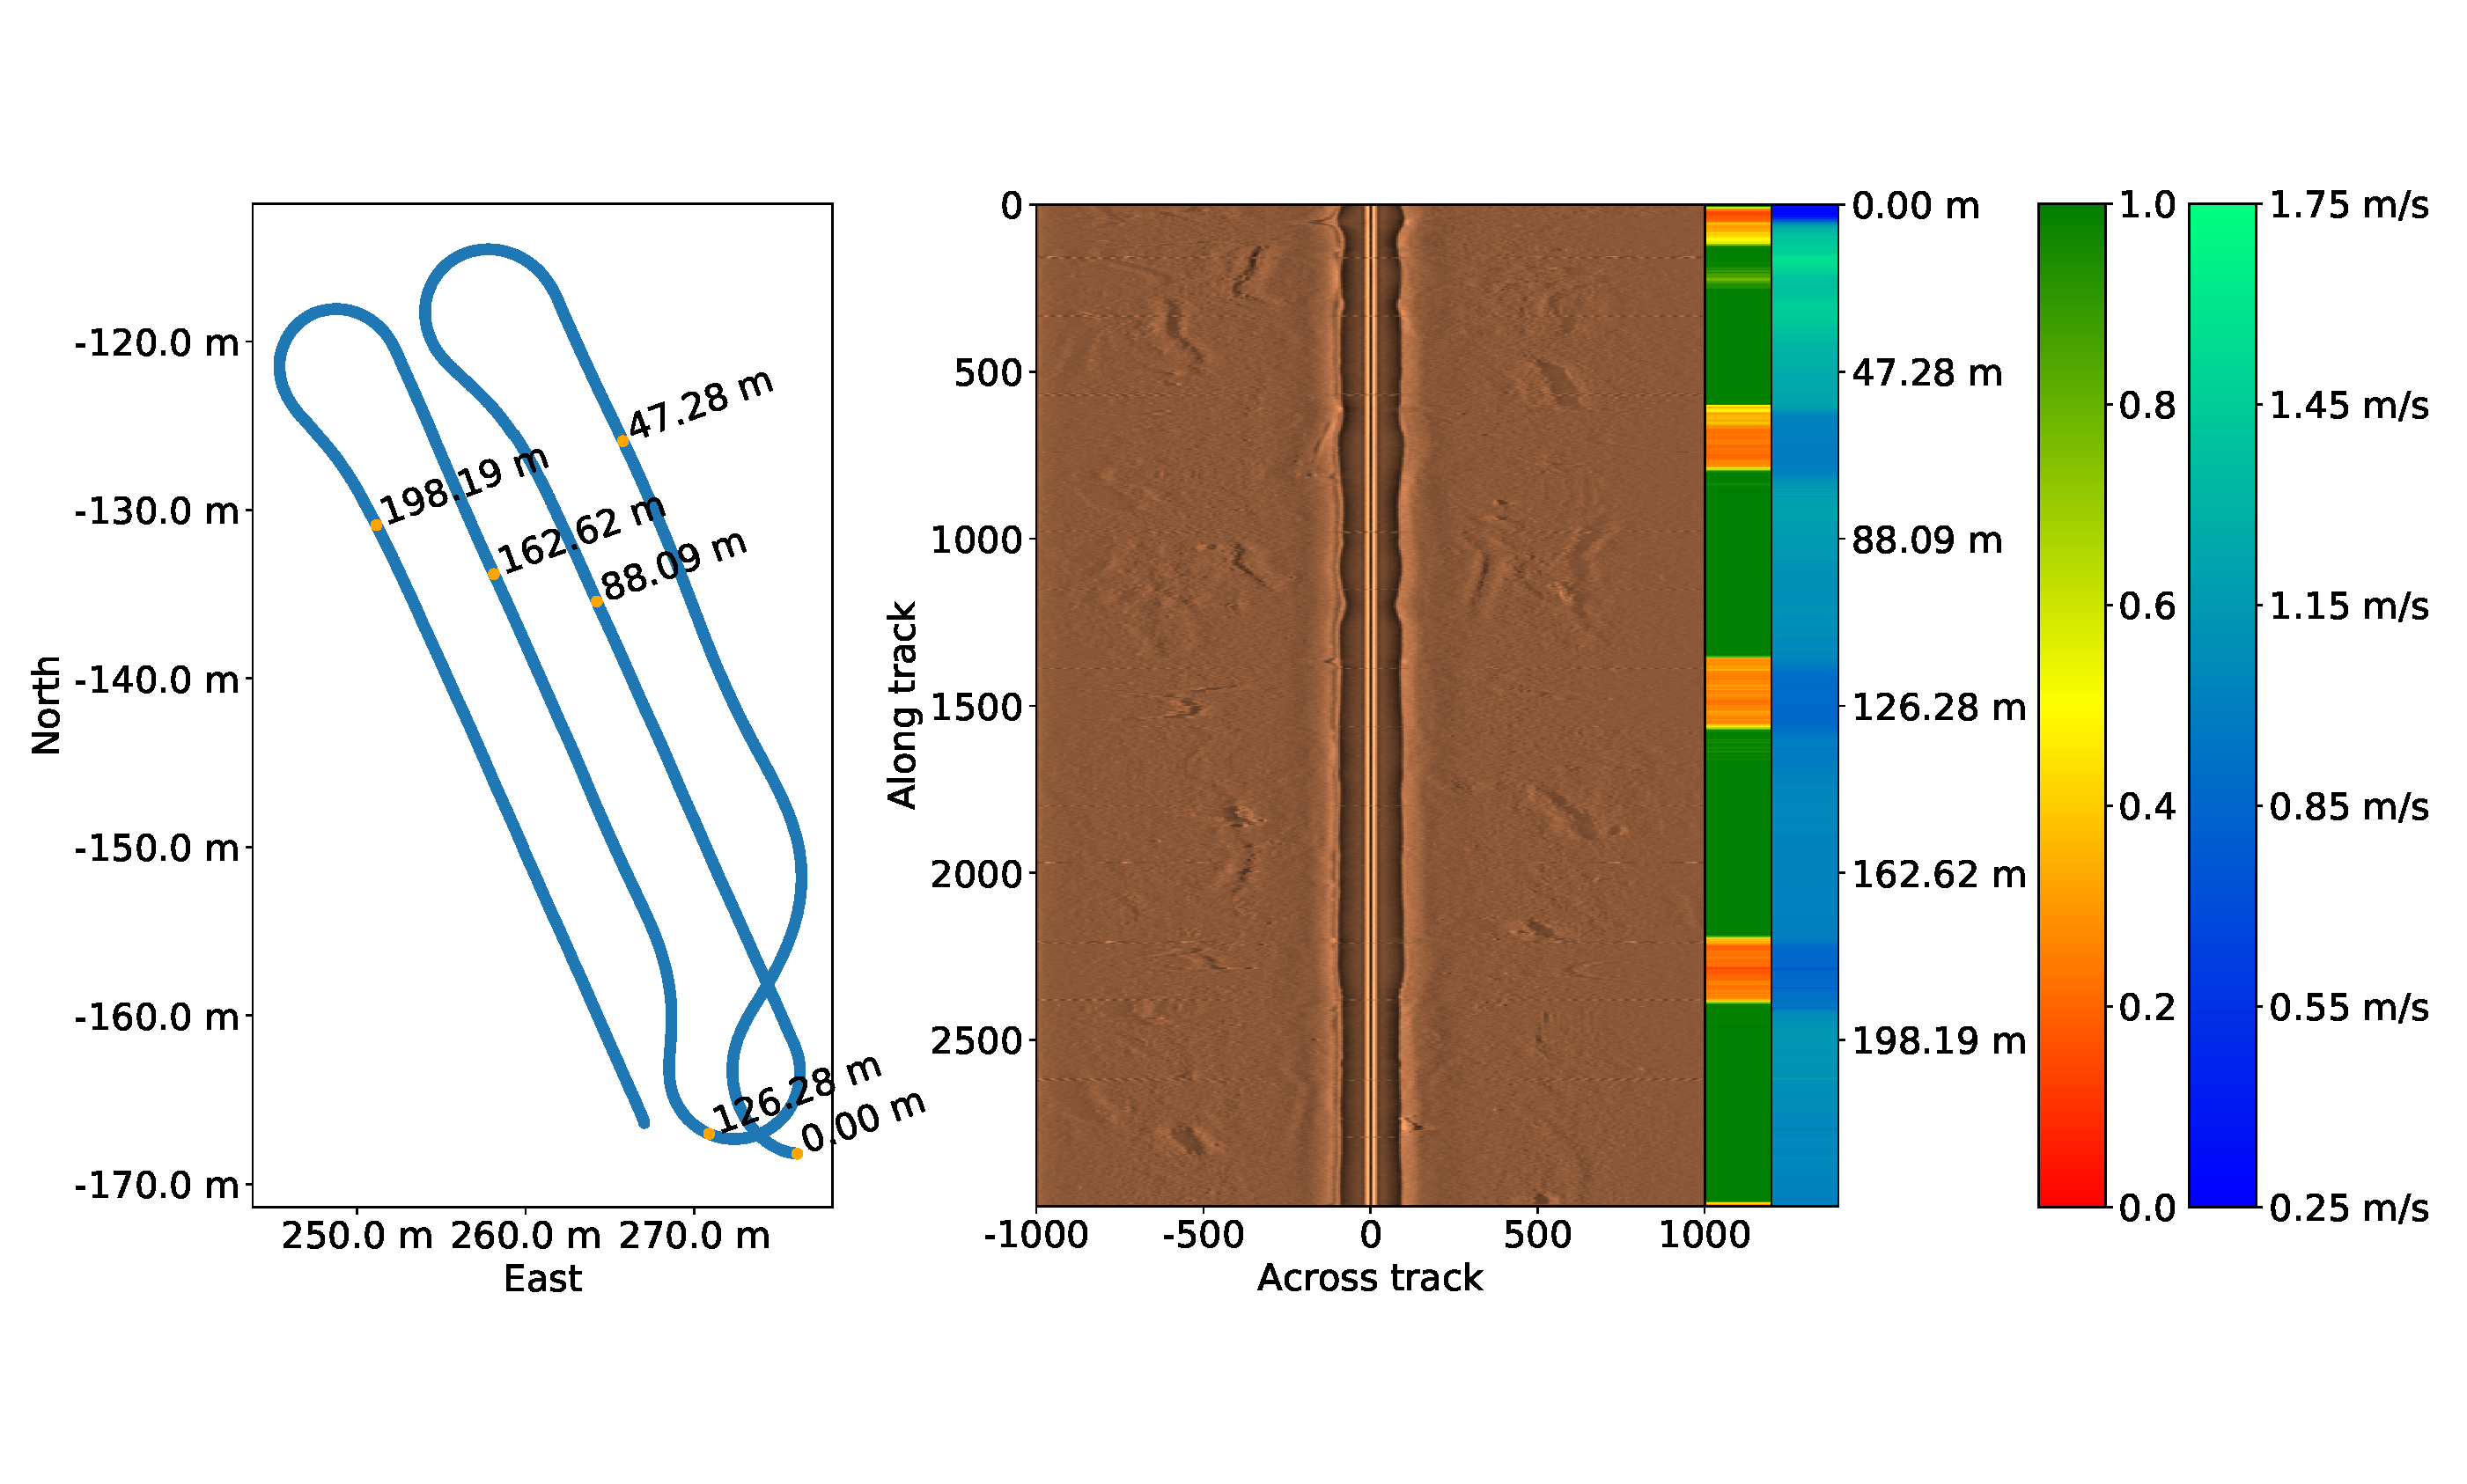
\includegraphics[trim=0cm 3.4cm 0cm 3.4cm, clip=true, width=\textwidth]{figures/path_sonar_colorbars_test.eps}
         \caption{\textbf{Left:} The traveled path of the AUV from the test data set. In addition, the traveled distance is shown along the path. \textbf{Right:} The acquired normalized sonar image, from the test data with its corresponding quality indicator and speed in the xy-plane showed in direct relation, respectively. The color scaling of the quality indicator and speed used for all test data is shown on the far right.}
         \label{fig:test_data}
     \end{subfigure}
     \hfill
     \begin{subfigure}[b]{0.44\textwidth}
         \centering
         \includegraphics[trim=9cm 1cm 10cm 1cm, clip=true, width=\textwidth]{figures/1D_norm_result_test.eps}
         \caption{1D landmark detector. Green is echo landmarks, and pink is shadow landmarks.}
         \label{fig:1D_norm_result_test}
     \end{subfigure}
     \begin{subfigure}[b]{0.44\textwidth}
         \centering
         \includegraphics[trim=9cm 1cm 10cm 1cm, clip=true, width=\textwidth]{figures/2D_result_single_test.eps}
         \caption{2D landmark detector. Pink is the detected landmarks.}
         \label{fig:2D_result_single_test}
     \end{subfigure}
        \caption{The test data represented and the results from running landmark detectors on the test data.}
        \label{fig:landmark_detection_test_data}
\end{figure}

\chapter{Discussion}

This chapter will discuss the results from the proposed landmark detectors and the quality indicator. In addition, a comparison of the two landmark detectors will be presented. 

\section{Quality Indicator for Side Scan Sonar}

The proposed quality indicator returns meaningful estimates of the dataset's quality and reports poor quality whenever the AUV turns, thus, we are able to point out the parts of the sonar image where anomalies are expected to occur. First, looking at the path in the top left part in \cref{fig:path_and_quality_ind}, it is shown that the quality indicator estimates poor quality whenever the AUV turns sharply. For the straightening up after a sharp turn, for example, at a traveled distance of $70 m$, no poor quality is reported. Even though it is a turn, it is not sharp enough to cause significant overlapping. On the other hand, inspecting the path around a traveled distance of $250 m$, we can again see that the AUV is straightening up after a sharp turn. However, the straightening up is slightly sharper, and a few yellow markers can be seen, indicating slight overlaps for a few swaths. 

Second, in the bottom part of \cref{fig:path_and_quality_ind}, where a part of the path is displayed with two and two consecutive effective ground ranges and "x"s marking the overlapping, it is shown how this overlapping affects the quality indicator. The closer the overlapping is to the AUV, the lower the estimated quality of the data. For no overlapping in the effective ground range, a quality indicator of $1.00$ is achieved. Looking at the swaths, we see how mapping these swaths to a sonar image will affect the image's appearance. For the part of the image that represents the outer turn, the spacing between each swath will be larger the further away from the AUV we get, effectively compressing objects and making them look smaller than their real size in the sonar image. For the inner turn, it is more complicated. Firstly, the part of the image from the AUV until the swaths overlap will appear enlarged. Second, the part from the point of overlap and away from the AUV will be flipped. Combining several swaths, we see how intertangled the information becomes with only a selection of six swaths. It is therefore expected that the image of the inner turn can present many different anomalies and that it will be hard to infer the information that appears. 

Finally, looking at the right sonar image in \cref{fig:path_and_quality_ind}, the black lines loosely divide the sonar image into good and poor-quality parts. The first to notice in the parts of poor quality (i.e., where the quality indicator differs from green in the image), most of the landmarks appear to be, as expected, distorted in some way. At around a traveled distance of $60 m$, a banana-formed landmark appears in both the left and right swath. The left swath is the outer turn, and we expect the banana-formed object to be compressed. Making basic geometric interpretations, we know that straight lines on the seafloor in the along-track direction will appear bent in the sonar image. It is likely that this has happened to the banana-formed landmark in the left swath. The right part of the swath is the inner turn, and it is therefore hard to infer anything from the information in the sonar image.

Even though the quality indicator can point out where distortion and poor quality can appear due to swath overlapping, it will to a lesser degree, be able to point out if we will experience distortions due to weak turning, change in speed, or a change in roll angle. Looking at \cref{fig:path_and_quality_ind} again, we can see that after turns one and three, there is a section where the AUV is straightening up and performing a weaker turn to approach its path. Looking at the corresponding parts of the right-side sonar image, it is evident that the image appears torn and much of the contrast disappears, especially in the left swath. The quality indicator marks a few swaths as weak yellow, but it is not a clear indicator of the torn image. In addition, since speed is not directly incorporated and roll isn't incorporated in the quality indicator, it will not be able to detect distortions from changes in these.

To summarise, we note that the indicator returns meaningful estimates when the situation is thought "easy", since it only infers on the overlapping of consecutive swaths and does not directly take into account changes in speed and the roll angle. The proposed indicator is thus brittle with respect to this situation, in the sense that it will provide non-reliable indications when anomalies in the data occur from changing speed or roll angle.  

\section{1D Landmark Detector using Peak Detection} \label{sec:disc_1D_landmark_detector}

As shown in \cref{fig:1D_norm_result_test}, the 1D landmark detector can detect some landmarks consistently, but most are not consistently detected. The top five landmarks are not close to being consistently detected. Two of the four landmarks at the bottom are consistently detected, and the last two are part of a larger landmark that is only partially consistently detected. If this landmark detection method should be used for SLAM, the data association would likely struggle to provide suitable landmark matches. 

Comparing the results in \cref{fig:1D_tuning_results}, it is evident that there is not much difference in the performance between using unnormalized and normalized data, but using normalized data in combination with morphological operators gives a significant increase in performance. Firstly, the choice between unnormalized and normalized data is not obvious from the tuning results, as there is an insignificant difference in the performance. However, normalized data have general advantages over unnormalized. Normalized data are the preferred choice because normalized data have the same intensity properties over the whole swath, making it possible to expect the same detection performance over the whole swath, as unnormalized has a great difference in dynamic range across track. Further, because of the significant increase in performance, utilizing morphological operators on the normalized data is also the preferred choice. However, to filter out the thin landmarks and increase the consistency of the detected landmarks, much of the geometrical details and information are filtered out, not providing much more information than the position of the landmarks and, to some extent, their size. Depending on the application, this may be sufficient. Still, for use in a SLAM pipeline, the landmark detector should be able to extract as much information from the landmarks as possible. If it turns out that the information isn't needed further down the pipeline, it can easily be filtered out. 

The process of tuning the 1D landmark detector was complex due to the parameters being tightly coupled and unintuitive since there was no direct relation between the threshold parameter and the desired properties of the detector. The latter can be seen in \cref{fig:1D_raw_tuning_training}, where three different thresholds are shown and compared to the chosen threshold of $E = 17$. A threshold of $E = 18$ makes some landmarks more consistent but also introduces a new echo landmark that is not consistently detected around swath number $400$. On the other hand, with a threshold of $16$, only one echo landmark is removed around swath number $1700$, but the others do not seem to get more consistent. Throughout the tuning process, it became evident that it was very hard to sort out the landmarks of the desired size, as both small and large landmarks were added or removed if the threshold was altered. It was also evident that there was a tight coupling between the smoothing parameter and the threshold. A change in the smoothing parameter implied that the range where the threshold parameter gave somewhat acceptable results vas drastically change, making the tuning more complex. 

To sum up, the 1D landmark method cannot detect landmarks consistently and, at the same time, produce an acceptable amount of false positives and is, therefore, not usable in any practical application. In addition, its tuning process is complex and unintuitive, and the best parameter set found filtered out a lot of the geometrical information about the landmarks. 

\section{2D Landmark Detector using Expert Rules}

As shown in \cref{fig:2D_result_single_test}, the 2D method can, to a larger extent, detect consistent or near-consistent landmarks in the data, but still, not all detected landmarks are consistent. From the top, the first landmark is inconsistently detected. In addition, landmark number four from the top appears to be close to consistent, but it is hard to point out what would be the ground truth for the landmark. The remaining landmarks are consistently detected. Therefore, even though not all landmarks are detected perfectly consistently, the method overall shows acceptable performance.

The tuning process is simple and mostly intuitive, as shown in \cref{fig:2D_tuning_intensity_thres} and \cref{fig:2d_tuning_paramaters_training}, and we can easily tune the different parameters to filter out the landmarks with the wanted geometrical properties. Because of the sequential inner workings of the detector, the tuning can also be done sequentially, making it possible to tune one parameter at a time. First, the intensity is tuned to pick out all landmarks consistently, together with an acceptable amount of false positives. The effect of the different intensity thresholds on the consistency and amount of false positives is easily observed in \cref{fig:2D_tuning_intensity_thres}. Next, the different geometrical parameters can be tuned to filter out the landmarks with the desired geometrical properties. The height parameters and the fill rate threshold are easily interpretable, and it is easy to predict their effect on the results. The area filtering is a bit more complex, as the area is corrected for the effect of the grazing angle. It is, therefore, not perfectly intuitive how it will affect the landmarks because its effect varies with how far the landmarks are from the AUV. However, producing an acceptable result without intuition about how the parameter affected the result is not difficult. All in all, the tuning can be said to be simple and mostly intuitive. 

To conclude, the 2D landmark detector produces acceptable results and possesses properties that make it simple and intuitive to tune, but it has some weaknesses regarding consistent landmark detection. Further work could improve the latter by doing a new local detection around each detected landmark with a relaxed intensity threshold to improve consistency.

\section{Comparison}

Both landmark detection methods can do detection with an acceptable level of false positives but suffer, to a varying degree, from not being able to detect the detected landmarks consistently. The 1D landmark detector struggles much more with consistently detecting landmarks than the 2D landmark detector and is considered unable to use in a practical application. The 2D landmark detector, on the other hand, has a much better performance and the potential to be used in practical applications.  However, inconsistent landmarks detection will make it much more challenging to apply in a SLAM context.

Even though the 2D landmark detector has almost twice as many tuning parameters, it is less complex and more intuitive to tune than the 1D landmark detector. This comes from the sequential inner workings and the non-dependent tuning parameters. The tuning is also worth considering for practical applications and, again, has the 2D landmark detector potential for being used in a SLAM context. 

\chapter{Conclusions and further work}

This report tested two different landmark detection methods for SSS, qualitatively compared them against each other, and presented a novel quality indicator for SSS data. 

The main findings may be summarized as follows: first of all, with respect to the 1D landmark detector, which uses peak detection to find shadows and echoes in 1D sonar swaths, we noted how adding morphological operators effectively removes false positives and increases its consistency. At the same time making this addition also leads to filtering out much of the geometrical information about the landmarks. However, even with increased consistency, it seems it cannot achieve acceptable performance and we deem it therefore unusable in the context of feature-based SLAM.

The second method, which finds shadows in 2D sonar images using expert rules, also increases its performance as soon as one uses morphological operators (more precisely, increasing its consistency). Though our experiments have shown that this 2D landmark detector cannot consistently detect all landmarks - the goals for the tuning were uncomplicated to achieve, thus not detecting any false positives and close to consistently detecting landmarks, deeming it an acceptable performance. We suggest that future works should thus focus on adapting such 2D landmark detector to be able to work on SSS data mapped to the cartesian space, making parameters filtering the landmarks based on their actual size. 

Finally, we comment on the here proposed quality indicator, which uses the information available in the dataset to infer its quality for the purposes of SLAM. We note that the indicator returns meaningful estimates when the situation is thought "easy", since it only infers on the overlapping of consecutive swaths and does not directly take into account changes in speed and the roll angle. The proposed indicator is thus brittle with respect to this situation, in the sense that it will provide non-reliable indications when anomalies in the data occur from changing speed or roll angle. Further work should thus focus on robustifying it, i.e., incorporating the effects of changes in speed and roll on the data. 

Further, we believe that it would be useful for both the academic and industrial communities to have an openly available dataset of benchmarks enabling the comparison of every method against a common ground.











\chapter*{\bibname}
\printbibliography[heading=none]

\appendix


\end{document}
